%% CS854 RadixVM Presentation
%% Winter 2016

%%% BEGIN PREAMBLE
\documentclass[aspectratio=169]{beamer}
\usepackage{hyperref}
\usepackage{color}
\usepackage{multirow}

%% Smart underlining -- from cdi-macros.tex
\def\ul#1{$\underline{\smash{\hbox{#1}}}$}

% TikZ packages (for graphs)
\usepackage{tkz-graph}
\usepackage{tkz-berge}
\usepackage{gnuplot-lua-tikz}
\usetikzlibrary{snakes}
\usetikzlibrary{backgrounds}

%% Shortcuts

\newcommand{\tabitem}{~~\llap{\textbullet}~~}

\newcommand\vm{RadixVM}
\newcommand\refcache{Refcache}

\newcommand{\bi}{\begin{itemize}}
\newcommand{\ei}{\end{itemize}}

\newcommand{\bn}{\begin{enumerate}}
\newcommand{\en}{\end{enumerate}}

\newcommand{\bd}{\begin{description}}
\newcommand{\ed}{\end{description}}

\mode<presentation>
{
  \usetheme{Madrid}
  \useinnertheme{circles}
  \usecolortheme{beaver}
}
\usepackage[english]{babel}

\usepackage{times}
\usepackage[T1]{fontenc}
% Note that the encoding and the font should match. If T1 does not
% look nice, try deleting the line with the fontenc.

\title{RadixVM}
\subtitle{Scalable address spaces for multithreaded applications}

\author[Presented by Simon Pratt]{Austin T. Clements,\\M. Frans Kaashoek,\\Nickolai Zeldovich\\
  \vspace{2em}Presented by Simon Pratt}

\date{February 12, 2016}


%%% BEGIN DOCUMENT
\begin{document}

\frame[plain]{\titlepage}

\begin{frame}{Abstract}
  \begin{columns}[T]
    \begin{column}{0.3\textwidth}
    \end{column}
    \begin{column}{0.4\textwidth}
      RadixVM solves 2 problems:
      \bn
      \pause
    \item Multithreaded address space scaling
      \bn
      \pause
    \item (And reference counting)
      \en
      \pause
    \item Remote TLB shootdown
      \en
      \vspace{2em}
      \pause
      But first, some background...
    \end{column}
    \begin{column}{0.3\textwidth}
    \end{column}
  \end{columns}
\end{frame}

\newpage

\section{Background}

\begin{frame}{Background: \texttt{malloc} and \texttt{mmap}}
  \begin{columns}[T]
    \begin{column}{0.2\textwidth}
      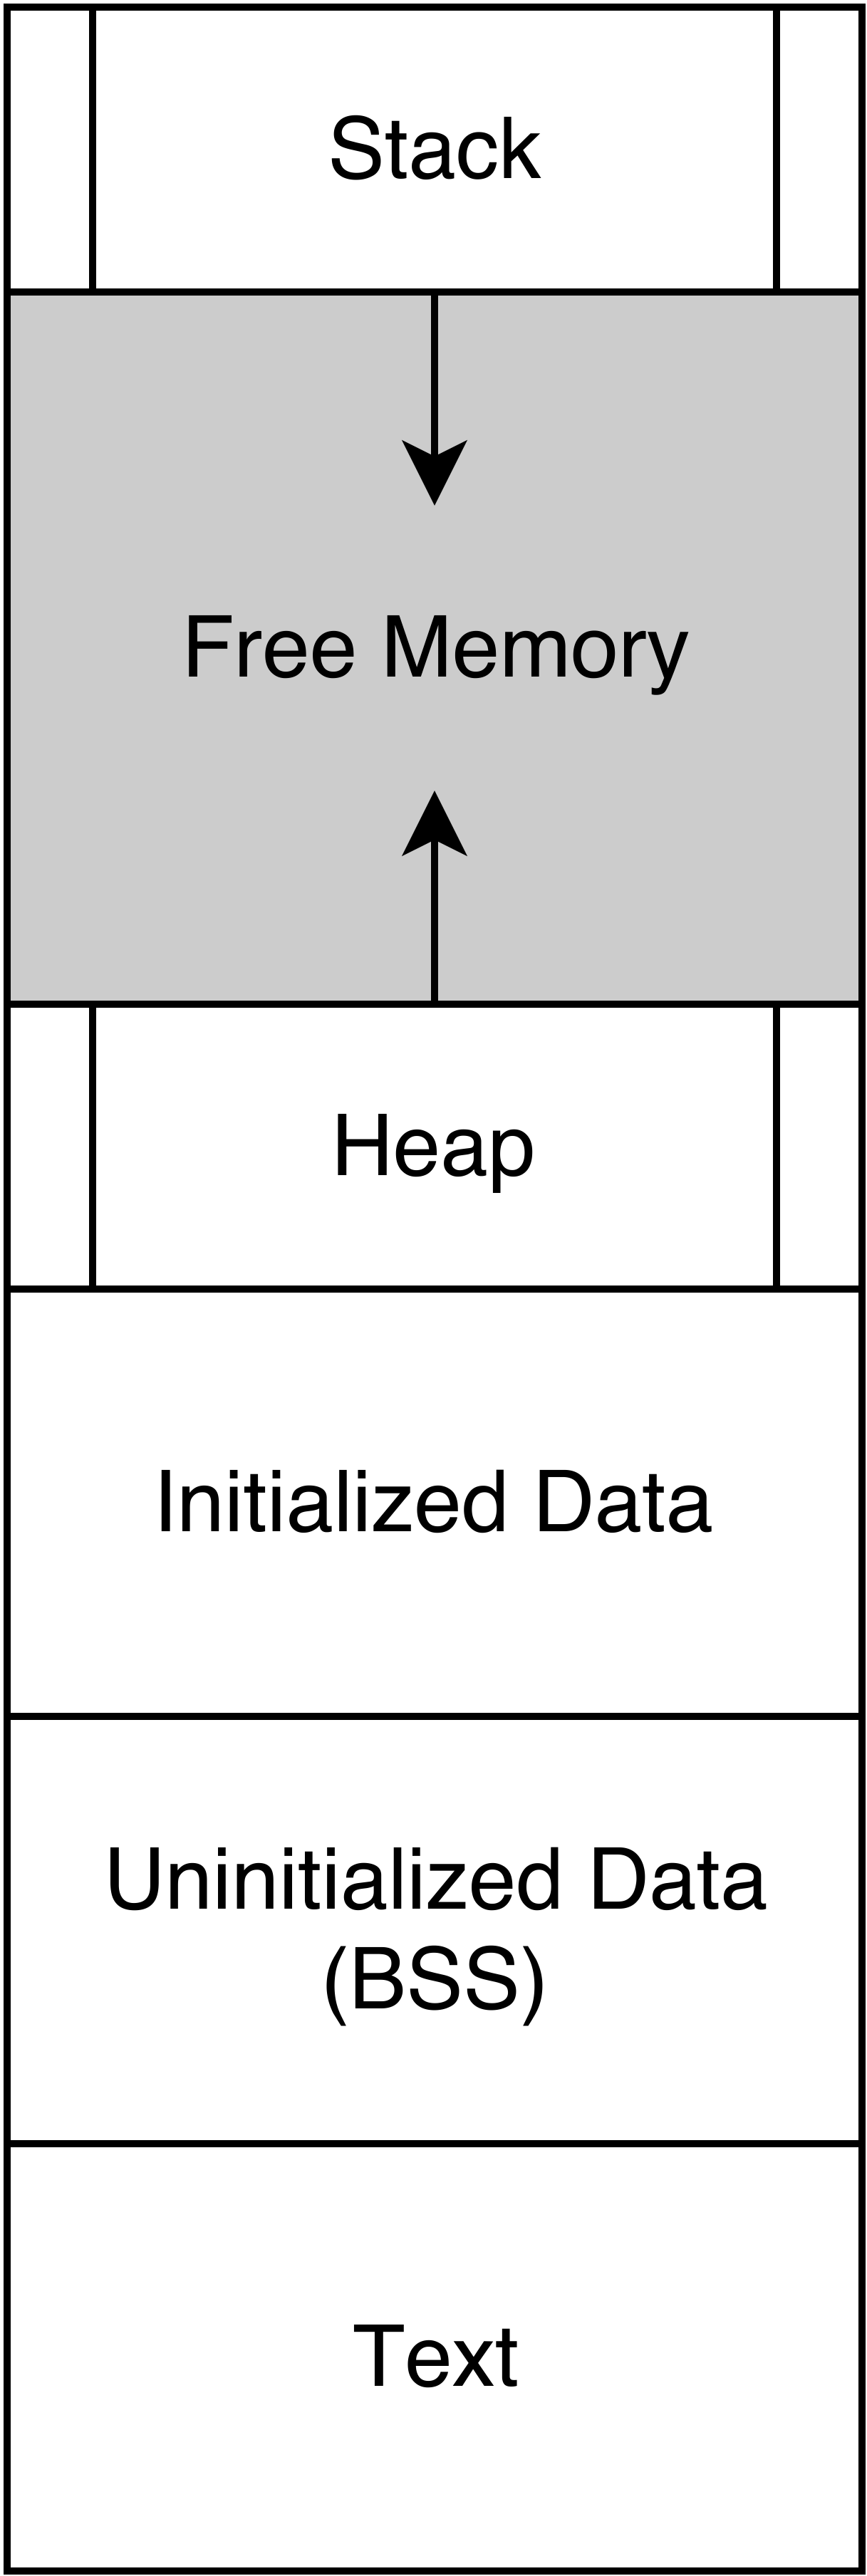
\includegraphics[scale=0.05]{./figures/Address_space.png}
    \end{column}
    \begin{column}{0.8\textwidth}
      \bi
    \item \texttt{malloc} and \texttt{free}
      \bi
    \item User-level library function
    \item Allocates/frees space in virtual memory
    \item Often implemented using \texttt{mmap} and \texttt{munmap}
      \ei
      \pause
    \item \texttt{mmap} and \texttt{munmap}
      \bi
    \item System calls
    \item Actually allocates/frees space in virtual memory
      \ei
      \pause
    \item So what is virtual memory?
      \ei
    \end{column}
  \end{columns}
\end{frame}

\begin{frame}{Background: Virtual Memory}
  \begin{columns}[T]
    \begin{column}{0.3\textwidth}
      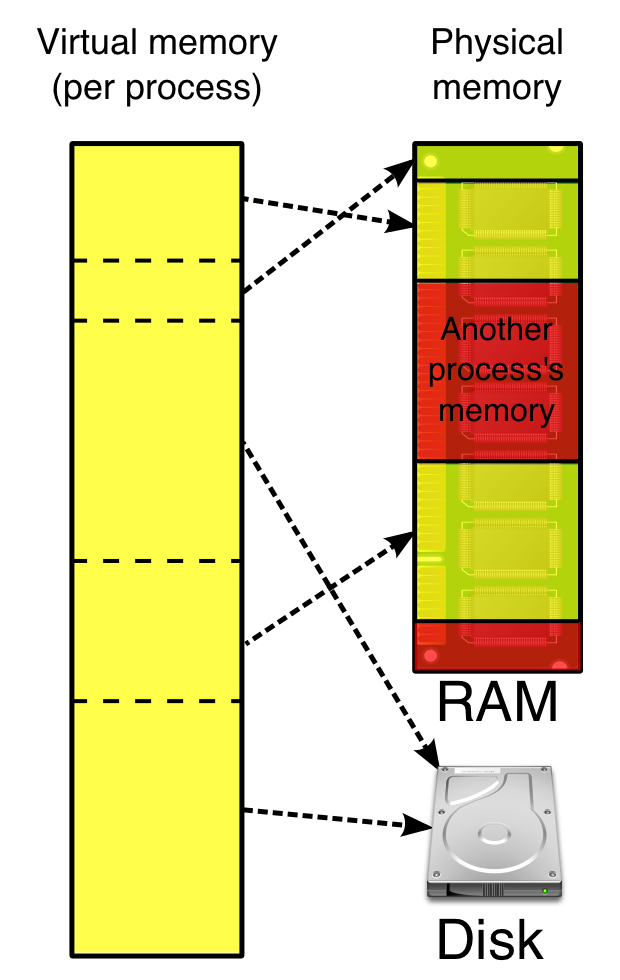
\includegraphics[scale=0.2]{./figures/Virtual_memory.png}
    \end{column}
    \begin{column}{0.7\textwidth}
      \bi
    \item (on x86) Instructions operate on virtual addresses
      \pause
    \item Data may be stored:
      \bi
    \item In physical memory
    \item On disk
      \ei
      \ei
    \end{column}
  \end{columns}
\end{frame}

\begin{frame}{Background: Virtual Memory}
  \begin{columns}[T]
    \begin{column}{0.5\textwidth}
      \vspace{-1em}
      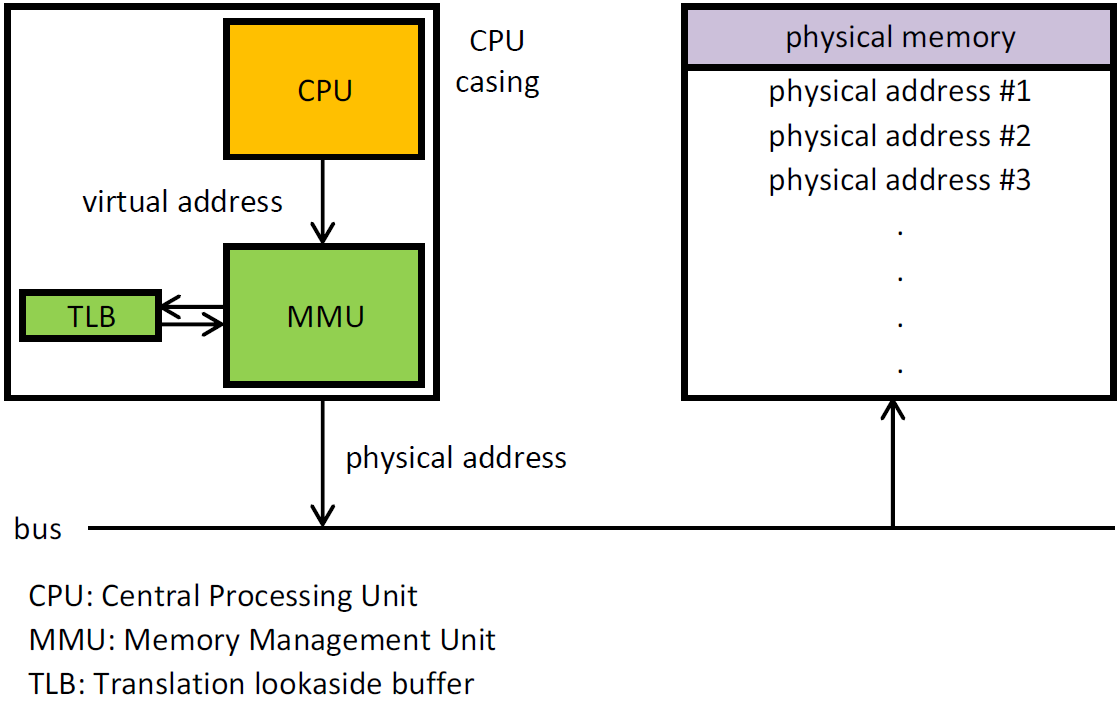
\includegraphics[scale=0.2]{./figures/MMU.png}
    \end{column}
    \begin{column}{0.5\textwidth}
      \vspace{5em}
      \bi
    \item Hardware, memory management unit (MMU)
      \bi
    \item Performs the translation
    \item Keeps a cache (TLB) of\\virtual $\rightarrow$ physical mappings
    \item No entry in TLB $\rightarrow$ page fault
      \ei
      \pause
    \item Operating system
      \bi
    \item Maintains the mapping (per process)
    \item Handles page faults
      \ei
      \pause
    \item So how does the OS store this?
      \ei
    \end{column}
  \end{columns}
\end{frame}

\begin{frame}{Background: Linux Virtual Memory}
  \begin{center}
    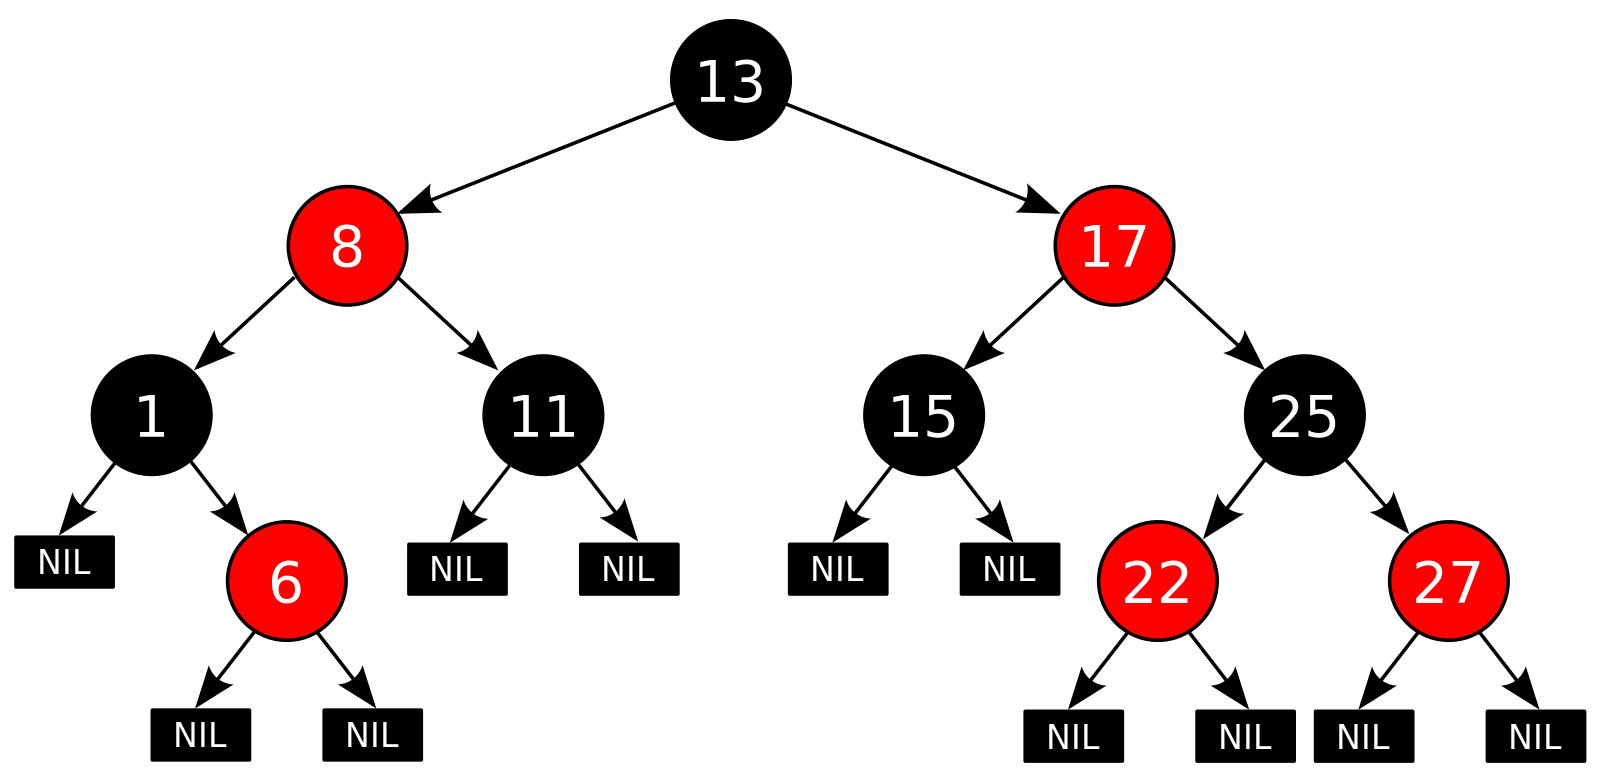
\includegraphics[scale=0.2]{./figures/Red-black_tree.png}
  \end{center}
    \bi
    \item Red-black tree
    \item Allows the kernel to search for memory area covering a virtual address
      \pause
    \item {\color{red}Problem: A single lock per address space!}
    \ei
\end{frame}

\begin{frame}{Problem 1: Multithreaded Address Space Scaling}
  \begin{center}
    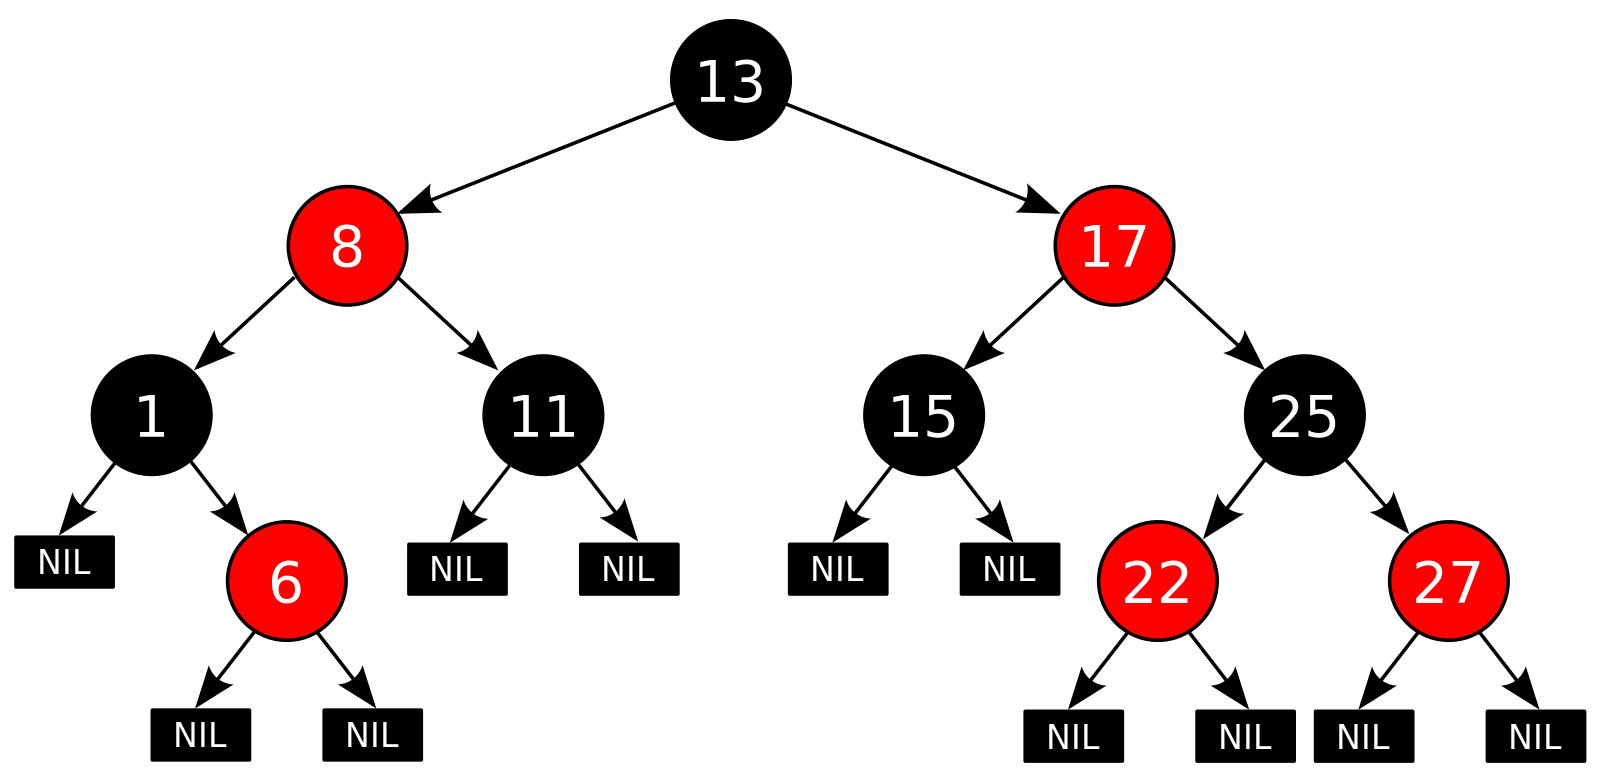
\includegraphics[scale=0.2]{./figures/Red-black_tree.png}
  \end{center}
    \bi
  \item {\color{red}A single lock on this structure} $\rightarrow$ \texttt{mmap} within a single process is serialized
    \pause
    \item Aside: prwlock paper notes that Psearchy is \texttt{mmap}-intensive
    \ei
\end{frame}

\begin{frame}{Abstract}
  \begin{columns}[T]
    \begin{column}{0.3\textwidth}
    \end{column}
    \begin{column}{0.4\textwidth}
      RadixVM solves 2 problems:
      \bn
    \item {\color<2>{red}Multithreaded address space scaling}
      \bn
    \item (And reference counting)
      \en
    \item Remote TLB shootdown
      \en
    \end{column}
    \begin{column}{0.3\textwidth}
    \end{column}
  \end{columns}
\end{frame}

\section{Design}

\begin{frame}{Background: Radix Tree}
  \begin{columns}[T]
    \begin{column}{0.5\textwidth}
      \begin{center}
        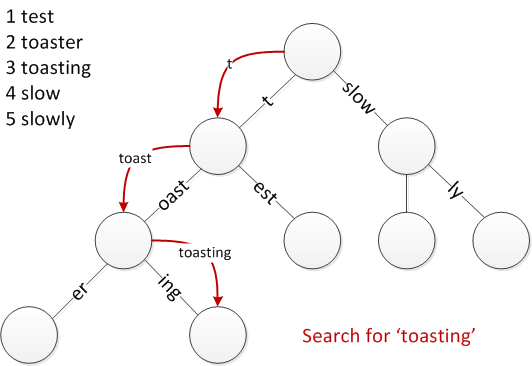
\includegraphics[scale=0.6]{./figures/Patricia_trie.png}
      \end{center}
    \end{column}
    \begin{column}{0.5\textwidth}
      \bi
    \item A.K.A. prefix tree
      \pause
    \item Edges labeled
      \pause
    \item Concatenation of edge labels along root$\rightarrow$node path gives a string
      \pause
    \item In OSes, usually strings of bits
      \ei
    \end{column}
  \end{columns}
\end{frame}

\begin{frame}{Design: RadixVM Data Structure}
  \begin{center}
  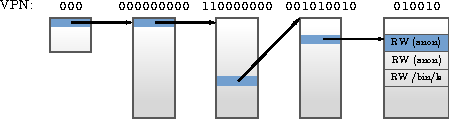
\includegraphics[scale=1.5]{./figures/radix.pdf}
  \end{center}
  \begin{columns}[T]
    \begin{column}{0.2\textwidth}
    \end{column}
    \begin{column}{0.6\textwidth}
      \bi
    \item Pretty much a page table
      \pause
    \item Each level indexed by up to 9 bits
      \pause
    \item Fixed-height $\rightarrow$ no balancing needed
      \pause
    \item Lazy expansion/collapsing
      \ei
    \end{column}
    \begin{column}{0.2\textwidth}
    \end{column}
  \end{columns}
\end{frame}

\begin{frame}{Design: RadixVM Data Structure}
  \begin{center}
  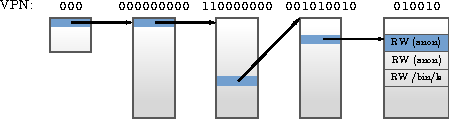
\includegraphics[scale=1.5]{./figures/radix.pdf}
  \end{center}
  \begin{columns}[T]
    \begin{column}{0.2\textwidth}
    \end{column}
    \begin{column}{0.6\textwidth}
      \bi
    \item Minimizes cache-line contention
      \pause
    \item Supports precise range locking
      \ei
    \end{column}
    \begin{column}{0.2\textwidth}
    \end{column}
  \end{columns}
\end{frame}

\begin{frame}{Problem 1.1: When to Free}
  \begin{center}
  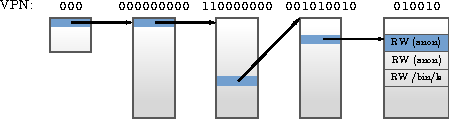
\includegraphics[scale=1.5]{./figures/radix.pdf}
  \end{center}
  \begin{columns}[T]
    \begin{column}{0.2\textwidth}
    \end{column}
    \begin{column}{0.6\textwidth}
      \bi
    \item How do we know when we can free the underlying pages?
      \pause
    \item Reference counting!
      \ei
    \end{column}
    \begin{column}{0.2\textwidth}
    \end{column}
  \end{columns}
\end{frame}

\begin{frame}{Abstract}
  \begin{columns}[T]
    \begin{column}{0.3\textwidth}
    \end{column}
    \begin{column}{0.4\textwidth}
      RadixVM solves 2 problems:
      \bn
    \item Multithreaded address space scaling
      \bn
    \item (And {\color<2>{red}reference counting})
      \en
    \item Remote TLB shootdown
      \en
    \end{column}
    \begin{column}{0.3\textwidth}
    \end{column}
  \end{columns}
\end{frame}

\begin{frame}{Background: Reference Counting}
  \begin{columns}[T]
    \begin{column}{0.1\textwidth}
        \vspace{2cm}
        \begin{tikzpicture}[node distance=1cm,overlay]
          \tikzstyle{every node}=[draw]
          % nodes
          \node<1-8> (M) {M};
          \node (T2) [below of=M] {$T_2$};
          \node (T1) [left of=T2] {$T_1$};
          \node (T3) [right of=T2] {$T_3$};
          % edges
          \draw<3-5> [->] (T1) to (M);
          \draw<4-6> [->] (T2) to (M);
          \draw<5-7> [->] (T3) to (M);
        \end{tikzpicture}
    \end{column}
    \begin{column}{0.6\textwidth}
      \bi
    \item 3 operations: inc, dec, zero?
      \pause
      \bn
    \item References: 0
      \pause
    \item inc $\rightarrow$ References: 1
      \pause
    \item inc $\rightarrow$ References: 2
      \pause
    \item inc $\rightarrow$ References: 3
      \pause
    \item dec $\rightarrow$ References: 2
      \pause
    \item dec $\rightarrow$ References: 1
      \pause
    \item dec $\rightarrow$ References: 0
      \pause
    \item zero? $\rightarrow$ Free M!
      \en
      \pause
    \item But: single counter $\rightarrow$ contention
      \ei
    \end{column}
  \end{columns}
\end{frame}

\begin{frame}{Design: Refcache}
  \begin{center}
  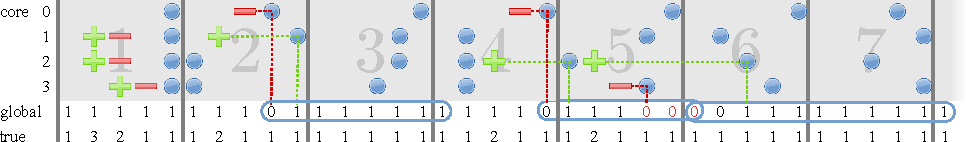
\includegraphics[scale=0.9]{./figures/refcache.pdf}
  \end{center}
  \begin{columns}[T]
    \begin{column}{0.4\textwidth}
    \end{column}
    \begin{column}{0.6\textwidth}
      \bi
    \item Per-core lazy counting
      \bi
      \pause
    \item Each core stores a delta
      \pause
    \item Delta updated lazily (blue circles)
      \ei
      \pause
    \item Divides time into epochs
      \pause
    \item Ref. count zero for an entire epoch $\rightarrow$ free
      \ei
    \end{column}
  \end{columns}
\end{frame}

\begin{frame}{Abstract}
  \begin{columns}[T]
    \begin{column}{0.3\textwidth}
    \end{column}
    \begin{column}{0.4\textwidth}
      RadixVM solves 2 problems:
      \bn
    \item Multithreaded address space scaling
      \bn
    \item (And reference counting)
      \en
    \item {\color<2>{red}Remote TLB shootdown}
      \en
    \end{column}
    \begin{column}{0.3\textwidth}
    \end{column}
  \end{columns}
\end{frame}

\begin{frame}{Problem 2: Remote TLB Shootdowns}
  \begin{columns}[T]
    \begin{column}{0.1\textwidth}
      \vspace{2cm}
      
\begin{tikzpicture}[node distance=1.5cm,overlay]
        \tikzstyle{every node}=[draw]
        % nodes 
        \node (M) {$M$};
        \node (P2) [above of=M] {$CPU_2$};
        \node (P4) [below of=M] {$CPU_4$};
        \node (P1) [left of=P2,node distance=1.5cm] {$CPU_1$};
        \node (P3) [left of=P4,node distance=1.5cm] {$CPU_3$};
        % edges
        \draw<1-3> [->,snake=snake] (P1) to (M);
        \draw<1-6> [->,snake=snake] (P3) to (M);
        \draw<6-> [->,blue] (P1) to (P2);
        \draw<6-> [->,blue] (P1) to (P3);
        \draw<6-> [->,blue] (P1) to (P4);
      \end{tikzpicture}
    \end{column}
    \begin{column}{0.5\textwidth}
      \bi
    \item Processes on $CPU_1$ and $CPU_3$ share memory area $M$
      \pause
    \item A process on $CPU_1$ unmaps $M$
      \bi
      \pause
    \item Flush local TLB entry
      \pause
      \pause
    \item Flush remote TLB entries\\(of anyone sharing)
      \ei
      \pause
    \item Linux: sends a {\color{blue}message} to all $CPU$
      \pause
      \pause
    \item \color{red}{This is expensive!}
      \ei
    \end{column}
  \end{columns}
\end{frame}

\begin{frame}{Design: Targeted TLB Shootdowns}
  \begin{columns}[T]
    \begin{column}{0.1\textwidth}
      \vspace{2cm}
      
\begin{tikzpicture}[node distance=1.5cm,overlay]
        \tikzstyle{every node}=[draw]
        % nodes 
        \node (M) {$M$};
        \node (P2) [above of=M] {$CPU_2$};
        \node (P4) [below of=M] {$CPU_4$};
        \node (P1) [left of=P2,node distance=1.5cm] {$CPU_1$};
        \node (P3) [left of=P4,node distance=1.5cm] {$CPU_3$};
        % edges
        \draw<1-2> [->,snake=snake] (P1) to (M);
        \draw<1-2> [->,snake=snake] (P3) to (M);
        \draw<2-> [->,blue] (P1) to (P3);
      \end{tikzpicture}
    \end{column}
    \begin{column}{0.5\textwidth}
      \bi
    \item Store metadata on which cores may have address in TLB
      \pause
    \item Only {\color{blue}flush} TLBs on cores which may share that memory
      \pause
      \ei
    \end{column}
  \end{columns}
\end{frame}

\section{Evaluation}

\begin{frame}{Implementation}
  \begin{columns}[T]
    \begin{column}{0.1\textwidth}
      \vspace{2cm}
      \begin{tikzpicture}[node distance=1.5cm,overlay]
        \tikzstyle{every node}=[draw]
        % nodes 
        \node<3-> (sv6) {sv6};
        \node<4-> (xv6) [below of=sv6] {xv6};
        \node<5-> (v6) [below of=xv6] {v6};
        % edges
        \draw<4-> [->] (sv6) to (xv6); 
        \draw<5-> [->] (xv6) to (v6); 
      \end{tikzpicture}
    \end{column}
    \begin{column}{0.6\textwidth}
      \bi
    \item \emph{Not} implemented on Linux
      \bi
      \pause
    \item Too complicated
      \ei
      \vspace{1em}
      \pause
    \item Implemented on sv6 (C++)
      \bi
      \pause
    \item Based on xv6 (ANSI C)
      \bi
      \pause
    \item Based on v6 Unix (K\&R C)
      \ei
      \pause
    \item Academic OS
      \pause
    \item \url{https://github.com/aclements/sv6}
      \ei
      \ei
    \end{column}
  \end{columns}
\end{frame}

\begin{frame}{Comparison}
  \begin{center}
    \bi
  \item Compared against:
    \bi
    \pause
  \item Default Linux
    \pause
  \item ``Bonsai''
    \ei
    \ei
  \end{center}
\end{frame}

\begin{frame}{Background: Bonsai}
  \begin{columns}[T]
    \begin{column}{0.6\textwidth}
      \begin{center}
        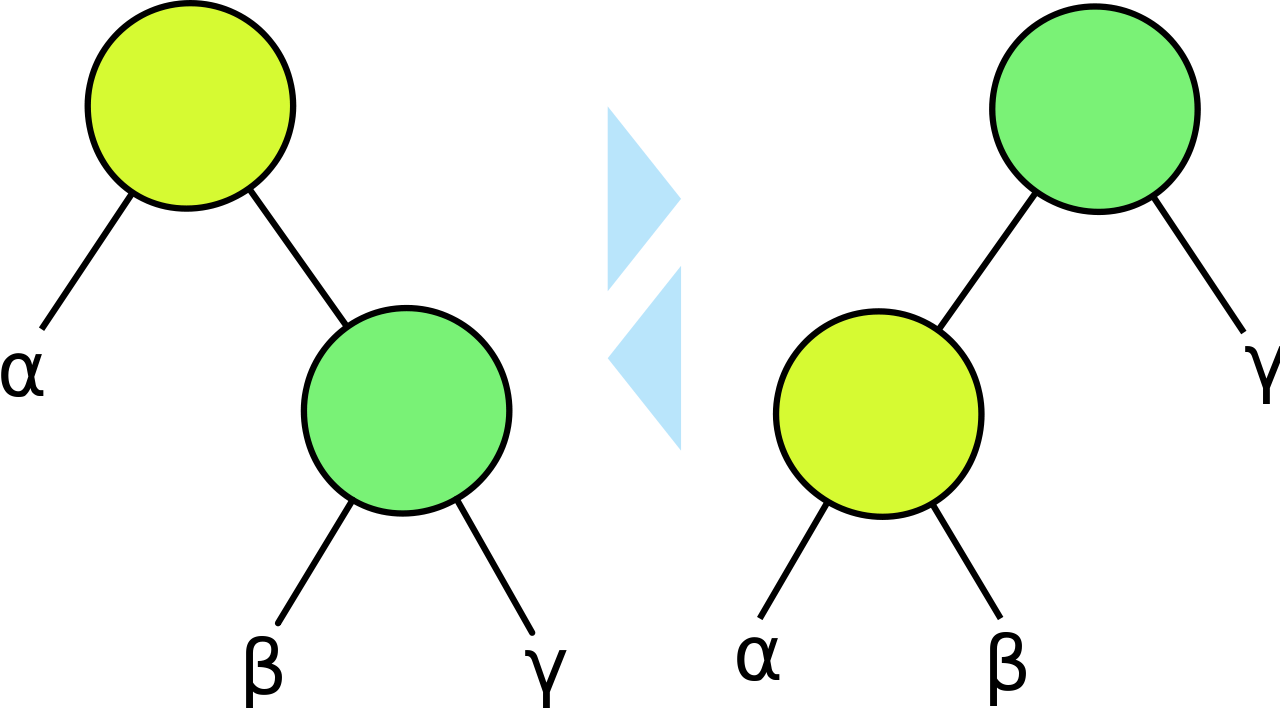
\includegraphics[scale=0.2]{./figures/Binary_tree_rotation.png}
      \end{center}
    \end{column}
    \begin{column}{0.4\textwidth}
      \bi
    \item Designed by the same authors
      \pause
    \item Uses an RCU-based balanced binary tree
      \pause
    \item Maintains bounded balance rather than strict balance\\
      (this means fewer rotations)
      \pause
    \item Rotations construct a new subtree rather than mutate the old one
      \ei
    \end{column}
  \end{columns}
\end{frame}

\begin{frame}{Application: Metis}
  \begin{columns}[T]
    \begin{column}{0.5\textwidth}
      \bi
    \item MapReduce Library
      \pause
    \item Single-server
      \pause
    \item Multithreaded
      \pause
    \item Stresses concurrent \texttt{mmap}s and \texttt{pagefault}s, but not concurrent \texttt{munmap}s
      \ei
    \end{column}
    \begin{column}{0.5\textwidth}
      \pause
      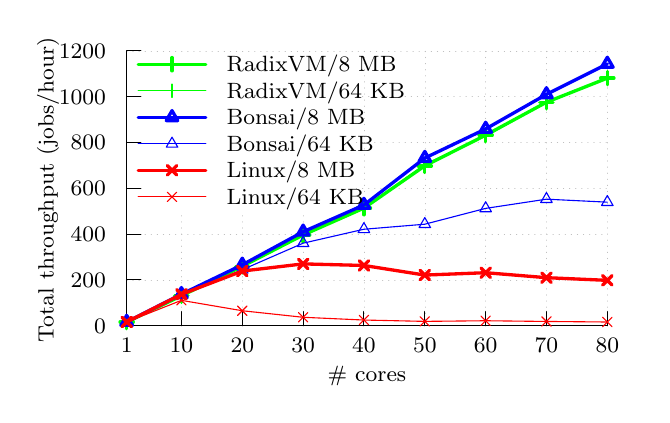
\begin{tikzpicture}[gnuplot]
%% generated with GNUPLOT 5.0p1 (Lua 5.3; terminal rev. 99, script rev. 100)
%% Tue  9 Feb 07:19:36 2016
\tikzset{every node/.append style={font={\fontsize{8.0pt}{9.6pt}\selectfont}}}
\path (0.000,0.000) rectangle (7.747,4.572);
\gpcolor{rgb color={0.753,0.753,0.753}}
\gpsetlinetype{gp lt axes}
\gpsetdashtype{gp dt axes}
\gpsetlinewidth{0.50}
\draw[gp path] (1.201,0.787)--(7.305,0.787);
\gpcolor{color=gp lt color border}
\gpsetlinetype{gp lt border}
\gpsetdashtype{gp dt solid}
\gpsetlinewidth{1.00}
\draw[gp path] (1.201,0.787)--(1.381,0.787);
\node[gp node right] at (1.054,0.787) {$0$};
\gpcolor{rgb color={0.753,0.753,0.753}}
\gpsetlinetype{gp lt axes}
\gpsetdashtype{gp dt axes}
\gpsetlinewidth{0.50}
\draw[gp path] (1.201,1.369)--(7.305,1.369);
\gpcolor{color=gp lt color border}
\gpsetlinetype{gp lt border}
\gpsetdashtype{gp dt solid}
\gpsetlinewidth{1.00}
\draw[gp path] (1.201,1.369)--(1.381,1.369);
\node[gp node right] at (1.054,1.369) {$200$};
\gpcolor{rgb color={0.753,0.753,0.753}}
\gpsetlinetype{gp lt axes}
\gpsetdashtype{gp dt axes}
\gpsetlinewidth{0.50}
\draw[gp path] (1.201,1.950)--(7.305,1.950);
\gpcolor{color=gp lt color border}
\gpsetlinetype{gp lt border}
\gpsetdashtype{gp dt solid}
\gpsetlinewidth{1.00}
\draw[gp path] (1.201,1.950)--(1.381,1.950);
\node[gp node right] at (1.054,1.950) {$400$};
\gpcolor{rgb color={0.753,0.753,0.753}}
\gpsetlinetype{gp lt axes}
\gpsetdashtype{gp dt axes}
\gpsetlinewidth{0.50}
\draw[gp path] (4.117,2.532)--(7.305,2.532);
\gpcolor{color=gp lt color border}
\gpsetlinetype{gp lt border}
\gpsetdashtype{gp dt solid}
\gpsetlinewidth{1.00}
\draw[gp path] (1.201,2.532)--(1.381,2.532);
\node[gp node right] at (1.054,2.532) {$600$};
\gpcolor{rgb color={0.753,0.753,0.753}}
\gpsetlinetype{gp lt axes}
\gpsetdashtype{gp dt axes}
\gpsetlinewidth{0.50}
\draw[gp path] (4.117,3.114)--(7.305,3.114);
\gpcolor{color=gp lt color border}
\gpsetlinetype{gp lt border}
\gpsetdashtype{gp dt solid}
\gpsetlinewidth{1.00}
\draw[gp path] (1.201,3.114)--(1.381,3.114);
\node[gp node right] at (1.054,3.114) {$800$};
\gpcolor{rgb color={0.753,0.753,0.753}}
\gpsetlinetype{gp lt axes}
\gpsetdashtype{gp dt axes}
\gpsetlinewidth{0.50}
\draw[gp path] (4.117,3.695)--(7.305,3.695);
\gpcolor{color=gp lt color border}
\gpsetlinetype{gp lt border}
\gpsetdashtype{gp dt solid}
\gpsetlinewidth{1.00}
\draw[gp path] (1.201,3.695)--(1.381,3.695);
\node[gp node right] at (1.054,3.695) {$1000$};
\gpcolor{rgb color={0.753,0.753,0.753}}
\gpsetlinetype{gp lt axes}
\gpsetdashtype{gp dt axes}
\gpsetlinewidth{0.50}
\draw[gp path] (1.201,4.277)--(7.305,4.277);
\gpcolor{color=gp lt color border}
\gpsetlinetype{gp lt border}
\gpsetdashtype{gp dt solid}
\gpsetlinewidth{1.00}
\draw[gp path] (1.201,4.277)--(1.381,4.277);
\node[gp node right] at (1.054,4.277) {$1200$};
\gpcolor{rgb color={0.753,0.753,0.753}}
\gpsetlinetype{gp lt axes}
\gpsetdashtype{gp dt axes}
\gpsetlinewidth{0.50}
\draw[gp path] (1.201,0.787)--(1.201,4.277);
\gpcolor{color=gp lt color border}
\gpsetlinetype{gp lt border}
\gpsetdashtype{gp dt solid}
\gpsetlinewidth{1.00}
\draw[gp path] (1.201,0.787)--(1.201,0.967);
\node[gp node center] at (1.201,0.541) {$1$};
\gpcolor{rgb color={0.753,0.753,0.753}}
\gpsetlinetype{gp lt axes}
\gpsetdashtype{gp dt axes}
\gpsetlinewidth{0.50}
\draw[gp path] (1.896,0.787)--(1.896,2.255);
\gpcolor{color=gp lt color border}
\gpsetlinetype{gp lt border}
\gpsetdashtype{gp dt solid}
\gpsetlinewidth{1.00}
\draw[gp path] (1.896,0.787)--(1.896,0.967);
\node[gp node center] at (1.896,0.541) {$10$};
\gpcolor{rgb color={0.753,0.753,0.753}}
\gpsetlinetype{gp lt axes}
\gpsetdashtype{gp dt axes}
\gpsetlinewidth{0.50}
\draw[gp path] (2.669,0.787)--(2.669,2.255);
\gpcolor{color=gp lt color border}
\gpsetlinetype{gp lt border}
\gpsetdashtype{gp dt solid}
\gpsetlinewidth{1.00}
\draw[gp path] (2.669,0.787)--(2.669,0.967);
\node[gp node center] at (2.669,0.541) {$20$};
\gpcolor{rgb color={0.753,0.753,0.753}}
\gpsetlinetype{gp lt axes}
\gpsetdashtype{gp dt axes}
\gpsetlinewidth{0.50}
\draw[gp path] (3.442,0.787)--(3.442,2.255);
\gpcolor{color=gp lt color border}
\gpsetlinetype{gp lt border}
\gpsetdashtype{gp dt solid}
\gpsetlinewidth{1.00}
\draw[gp path] (3.442,0.787)--(3.442,0.967);
\node[gp node center] at (3.442,0.541) {$30$};
\gpcolor{rgb color={0.753,0.753,0.753}}
\gpsetlinetype{gp lt axes}
\gpsetdashtype{gp dt axes}
\gpsetlinewidth{0.50}
\draw[gp path] (4.214,0.787)--(4.214,4.277);
\gpcolor{color=gp lt color border}
\gpsetlinetype{gp lt border}
\gpsetdashtype{gp dt solid}
\gpsetlinewidth{1.00}
\draw[gp path] (4.214,0.787)--(4.214,0.967);
\node[gp node center] at (4.214,0.541) {$40$};
\gpcolor{rgb color={0.753,0.753,0.753}}
\gpsetlinetype{gp lt axes}
\gpsetdashtype{gp dt axes}
\gpsetlinewidth{0.50}
\draw[gp path] (4.987,0.787)--(4.987,4.277);
\gpcolor{color=gp lt color border}
\gpsetlinetype{gp lt border}
\gpsetdashtype{gp dt solid}
\gpsetlinewidth{1.00}
\draw[gp path] (4.987,0.787)--(4.987,0.967);
\node[gp node center] at (4.987,0.541) {$50$};
\gpcolor{rgb color={0.753,0.753,0.753}}
\gpsetlinetype{gp lt axes}
\gpsetdashtype{gp dt axes}
\gpsetlinewidth{0.50}
\draw[gp path] (5.760,0.787)--(5.760,4.277);
\gpcolor{color=gp lt color border}
\gpsetlinetype{gp lt border}
\gpsetdashtype{gp dt solid}
\gpsetlinewidth{1.00}
\draw[gp path] (5.760,0.787)--(5.760,0.967);
\node[gp node center] at (5.760,0.541) {$60$};
\gpcolor{rgb color={0.753,0.753,0.753}}
\gpsetlinetype{gp lt axes}
\gpsetdashtype{gp dt axes}
\gpsetlinewidth{0.50}
\draw[gp path] (6.532,0.787)--(6.532,4.277);
\gpcolor{color=gp lt color border}
\gpsetlinetype{gp lt border}
\gpsetdashtype{gp dt solid}
\gpsetlinewidth{1.00}
\draw[gp path] (6.532,0.787)--(6.532,0.967);
\node[gp node center] at (6.532,0.541) {$70$};
\gpcolor{rgb color={0.753,0.753,0.753}}
\gpsetlinetype{gp lt axes}
\gpsetdashtype{gp dt axes}
\gpsetlinewidth{0.50}
\draw[gp path] (7.305,0.787)--(7.305,4.277);
\gpcolor{color=gp lt color border}
\gpsetlinetype{gp lt border}
\gpsetdashtype{gp dt solid}
\gpsetlinewidth{1.00}
\draw[gp path] (7.305,0.787)--(7.305,0.967);
\node[gp node center] at (7.305,0.541) {$80$};
\gpsetlinetype{gp lt axes}
\gpsetdashtype{gp dt axes}
\draw[gp path] (1.201,0.787)--(7.305,0.787);
\gpsetlinetype{gp lt border}
\gpsetdashtype{gp dt solid}
\draw[gp path] (1.201,4.277)--(1.201,0.787)--(7.305,0.787);
\node[gp node center,rotate=-270] at (0.196,2.532) {Total throughput (jobs/hour)};
\node[gp node center] at (4.253,0.172) {\# cores};
\node[gp node left] at (2.353,4.108) {\vm/8~MB};
\gpcolor{color=gp lt color 1}
\gpsetlinewidth{3.00}
\draw[gp path] (1.348,4.108)--(2.206,4.108);
\draw[gp path] (1.201,0.833)--(1.896,1.167)--(2.669,1.541)--(3.442,1.939)--(4.214,2.280)%
  --(4.987,2.817)--(5.760,3.207)--(6.532,3.625)--(7.305,3.931);
\gpsetpointsize{6.00}
\gppoint{gp mark 1}{(1.201,0.833)}
\gppoint{gp mark 1}{(1.896,1.167)}
\gppoint{gp mark 1}{(2.669,1.541)}
\gppoint{gp mark 1}{(3.442,1.939)}
\gppoint{gp mark 1}{(4.214,2.280)}
\gppoint{gp mark 1}{(4.987,2.817)}
\gppoint{gp mark 1}{(5.760,3.207)}
\gppoint{gp mark 1}{(6.532,3.625)}
\gppoint{gp mark 1}{(7.305,3.931)}
\gppoint{gp mark 1}{(1.777,4.108)}
\gpcolor{color=gp lt color border}
\node[gp node left] at (2.353,3.771) {\vm/64~KB};
\gpcolor{color=gp lt color 1}
\gpsetlinewidth{1.00}
\draw[gp path] (1.348,3.771)--(2.206,3.771);
\draw[gp path] (1.201,0.833)--(1.896,1.169)--(2.669,1.541)--(3.442,1.937)--(4.214,2.279)%
  --(4.987,2.836)--(5.760,3.193)--(6.532,3.618)--(7.305,3.926);
\gppoint{gp mark 1}{(1.201,0.833)}
\gppoint{gp mark 1}{(1.896,1.169)}
\gppoint{gp mark 1}{(2.669,1.541)}
\gppoint{gp mark 1}{(3.442,1.937)}
\gppoint{gp mark 1}{(4.214,2.279)}
\gppoint{gp mark 1}{(4.987,2.836)}
\gppoint{gp mark 1}{(5.760,3.193)}
\gppoint{gp mark 1}{(6.532,3.618)}
\gppoint{gp mark 1}{(7.305,3.926)}
\gppoint{gp mark 1}{(1.777,3.771)}
\gpcolor{color=gp lt color border}
\node[gp node left] at (2.353,3.434) {Bonsai/8~MB};
\gpcolor{color=gp lt color 2}
\gpsetlinewidth{3.00}
\draw[gp path] (1.348,3.434)--(2.206,3.434);
\draw[gp path] (1.201,0.834)--(1.896,1.187)--(2.669,1.560)--(3.442,1.980)--(4.214,2.320)%
  --(4.987,2.916)--(5.760,3.286)--(6.532,3.725)--(7.305,4.112);
\gppoint{gp mark 8}{(1.201,0.834)}
\gppoint{gp mark 8}{(1.896,1.187)}
\gppoint{gp mark 8}{(2.669,1.560)}
\gppoint{gp mark 8}{(3.442,1.980)}
\gppoint{gp mark 8}{(4.214,2.320)}
\gppoint{gp mark 8}{(4.987,2.916)}
\gppoint{gp mark 8}{(5.760,3.286)}
\gppoint{gp mark 8}{(6.532,3.725)}
\gppoint{gp mark 8}{(7.305,4.112)}
\gppoint{gp mark 8}{(1.777,3.434)}
\gpcolor{color=gp lt color border}
\node[gp node left] at (2.353,3.097) {Bonsai/64~KB};
\gpcolor{color=gp lt color 2}
\gpsetlinewidth{1.00}
\draw[gp path] (1.348,3.097)--(2.206,3.097);
\draw[gp path] (1.201,0.834)--(1.896,1.174)--(2.669,1.498)--(3.442,1.835)--(4.214,2.012)%
  --(4.987,2.076)--(5.760,2.277)--(6.532,2.394)--(7.305,2.356);
\gppoint{gp mark 8}{(1.201,0.834)}
\gppoint{gp mark 8}{(1.896,1.174)}
\gppoint{gp mark 8}{(2.669,1.498)}
\gppoint{gp mark 8}{(3.442,1.835)}
\gppoint{gp mark 8}{(4.214,2.012)}
\gppoint{gp mark 8}{(4.987,2.076)}
\gppoint{gp mark 8}{(5.760,2.277)}
\gppoint{gp mark 8}{(6.532,2.394)}
\gppoint{gp mark 8}{(7.305,2.356)}
\gppoint{gp mark 8}{(1.777,3.097)}
\gpcolor{color=gp lt color border}
\node[gp node left] at (2.353,2.760) {Linux/8~MB};
\gpcolor{color=gp lt color 0}
\gpsetlinewidth{3.00}
\draw[gp path] (1.348,2.760)--(2.206,2.760);
\draw[gp path] (1.201,0.834)--(1.896,1.185)--(2.669,1.481)--(3.442,1.572)--(4.214,1.552)%
  --(4.987,1.430)--(5.760,1.460)--(6.532,1.397)--(7.305,1.363);
\gppoint{gp mark 2}{(1.201,0.834)}
\gppoint{gp mark 2}{(1.896,1.185)}
\gppoint{gp mark 2}{(2.669,1.481)}
\gppoint{gp mark 2}{(3.442,1.572)}
\gppoint{gp mark 2}{(4.214,1.552)}
\gppoint{gp mark 2}{(4.987,1.430)}
\gppoint{gp mark 2}{(5.760,1.460)}
\gppoint{gp mark 2}{(6.532,1.397)}
\gppoint{gp mark 2}{(7.305,1.363)}
\gppoint{gp mark 2}{(1.777,2.760)}
\gpcolor{color=gp lt color border}
\node[gp node left] at (2.353,2.423) {Linux/64~KB};
\gpcolor{color=gp lt color 0}
\gpsetlinewidth{1.00}
\draw[gp path] (1.348,2.423)--(2.206,2.423);
\draw[gp path] (1.201,0.834)--(1.896,1.109)--(2.669,0.977)--(3.442,0.894)--(4.214,0.859)%
  --(4.987,0.842)--(5.760,0.850)--(6.532,0.841)--(7.305,0.834);
\gppoint{gp mark 2}{(1.201,0.834)}
\gppoint{gp mark 2}{(1.896,1.109)}
\gppoint{gp mark 2}{(2.669,0.977)}
\gppoint{gp mark 2}{(3.442,0.894)}
\gppoint{gp mark 2}{(4.214,0.859)}
\gppoint{gp mark 2}{(4.987,0.842)}
\gppoint{gp mark 2}{(5.760,0.850)}
\gppoint{gp mark 2}{(6.532,0.841)}
\gppoint{gp mark 2}{(7.305,0.834)}
\gppoint{gp mark 2}{(1.777,2.423)}
%% coordinates of the plot area
\gpdefrectangularnode{gp plot 1}{\pgfpoint{1.201cm}{0.787cm}}{\pgfpoint{7.305cm}{4.277cm}}
\end{tikzpicture}
%% gnuplot variables

    \end{column}
  \end{columns}
\end{frame}

\begin{frame}{Microbenchmark: Local}
  \begin{columns}[T]
    \begin{column}{0.5\textwidth}
      \bi
    \item \texttt{mmap} a private 4KB region in shared address space
      \pause
    \item Write to every page in region
      \pause
    \item \texttt{munmap} region
      \ei
    \end{column}
    \begin{column}{0.5\textwidth}
      \pause
      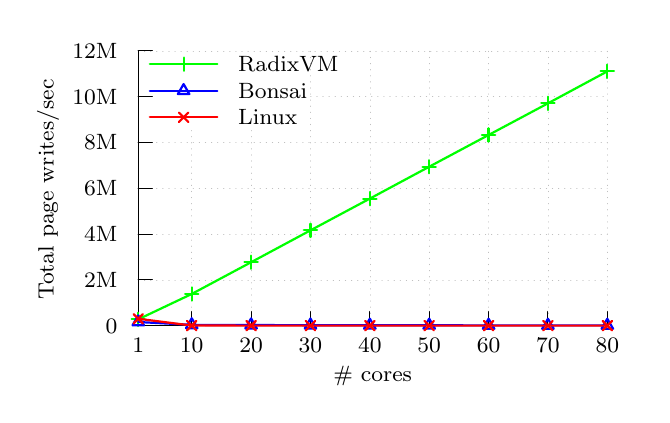
\begin{tikzpicture}[gnuplot]
%% generated with GNUPLOT 5.0p1 (Lua 5.3; terminal rev. 99, script rev. 100)
%% Tue  9 Feb 07:20:53 2016
\tikzset{every node/.append style={font={\fontsize{8.0pt}{9.6pt}\selectfont}}}
\path (0.000,0.000) rectangle (7.747,4.572);
\gpcolor{rgb color={0.753,0.753,0.753}}
\gpsetlinetype{gp lt axes}
\gpsetdashtype{gp dt axes}
\gpsetlinewidth{0.50}
\draw[gp path] (1.348,0.787)--(7.305,0.787);
\gpcolor{color=gp lt color border}
\gpsetlinetype{gp lt border}
\gpsetdashtype{gp dt solid}
\gpsetlinewidth{1.00}
\draw[gp path] (1.348,0.787)--(1.528,0.787);
\node[gp node right] at (1.201,0.787) {  0 };
\gpcolor{rgb color={0.753,0.753,0.753}}
\gpsetlinetype{gp lt axes}
\gpsetdashtype{gp dt axes}
\gpsetlinewidth{0.50}
\draw[gp path] (1.348,1.369)--(7.305,1.369);
\gpcolor{color=gp lt color border}
\gpsetlinetype{gp lt border}
\gpsetdashtype{gp dt solid}
\gpsetlinewidth{1.00}
\draw[gp path] (1.348,1.369)--(1.528,1.369);
\node[gp node right] at (1.201,1.369) {  2M};
\gpcolor{rgb color={0.753,0.753,0.753}}
\gpsetlinetype{gp lt axes}
\gpsetdashtype{gp dt axes}
\gpsetlinewidth{0.50}
\draw[gp path] (1.348,1.950)--(7.305,1.950);
\gpcolor{color=gp lt color border}
\gpsetlinetype{gp lt border}
\gpsetdashtype{gp dt solid}
\gpsetlinewidth{1.00}
\draw[gp path] (1.348,1.950)--(1.528,1.950);
\node[gp node right] at (1.201,1.950) {  4M};
\gpcolor{rgb color={0.753,0.753,0.753}}
\gpsetlinetype{gp lt axes}
\gpsetdashtype{gp dt axes}
\gpsetlinewidth{0.50}
\draw[gp path] (1.348,2.532)--(7.305,2.532);
\gpcolor{color=gp lt color border}
\gpsetlinetype{gp lt border}
\gpsetdashtype{gp dt solid}
\gpsetlinewidth{1.00}
\draw[gp path] (1.348,2.532)--(1.528,2.532);
\node[gp node right] at (1.201,2.532) {  6M};
\gpcolor{rgb color={0.753,0.753,0.753}}
\gpsetlinetype{gp lt axes}
\gpsetdashtype{gp dt axes}
\gpsetlinewidth{0.50}
\draw[gp path] (1.348,3.114)--(7.305,3.114);
\gpcolor{color=gp lt color border}
\gpsetlinetype{gp lt border}
\gpsetdashtype{gp dt solid}
\gpsetlinewidth{1.00}
\draw[gp path] (1.348,3.114)--(1.528,3.114);
\node[gp node right] at (1.201,3.114) {  8M};
\gpcolor{rgb color={0.753,0.753,0.753}}
\gpsetlinetype{gp lt axes}
\gpsetdashtype{gp dt axes}
\gpsetlinewidth{0.50}
\draw[gp path] (3.382,3.695)--(7.305,3.695);
\gpcolor{color=gp lt color border}
\gpsetlinetype{gp lt border}
\gpsetdashtype{gp dt solid}
\gpsetlinewidth{1.00}
\draw[gp path] (1.348,3.695)--(1.528,3.695);
\node[gp node right] at (1.201,3.695) {  10M};
\gpcolor{rgb color={0.753,0.753,0.753}}
\gpsetlinetype{gp lt axes}
\gpsetdashtype{gp dt axes}
\gpsetlinewidth{0.50}
\draw[gp path] (1.348,4.277)--(7.305,4.277);
\gpcolor{color=gp lt color border}
\gpsetlinetype{gp lt border}
\gpsetdashtype{gp dt solid}
\gpsetlinewidth{1.00}
\draw[gp path] (1.348,4.277)--(1.528,4.277);
\node[gp node right] at (1.201,4.277) {  12M};
\gpcolor{rgb color={0.753,0.753,0.753}}
\gpsetlinetype{gp lt axes}
\gpsetdashtype{gp dt axes}
\gpsetlinewidth{0.50}
\draw[gp path] (1.348,0.787)--(1.348,4.277);
\gpcolor{color=gp lt color border}
\gpsetlinetype{gp lt border}
\gpsetdashtype{gp dt solid}
\gpsetlinewidth{1.00}
\draw[gp path] (1.348,0.787)--(1.348,0.967);
\node[gp node center] at (1.348,0.541) {$1$};
\gpcolor{rgb color={0.753,0.753,0.753}}
\gpsetlinetype{gp lt axes}
\gpsetdashtype{gp dt axes}
\gpsetlinewidth{0.50}
\draw[gp path] (2.027,0.787)--(2.027,3.266);
\gpcolor{color=gp lt color border}
\gpsetlinetype{gp lt border}
\gpsetdashtype{gp dt solid}
\gpsetlinewidth{1.00}
\draw[gp path] (2.027,0.787)--(2.027,0.967);
\node[gp node center] at (2.027,0.541) {$10$};
\gpcolor{rgb color={0.753,0.753,0.753}}
\gpsetlinetype{gp lt axes}
\gpsetdashtype{gp dt axes}
\gpsetlinewidth{0.50}
\draw[gp path] (2.781,0.787)--(2.781,3.266);
\gpcolor{color=gp lt color border}
\gpsetlinetype{gp lt border}
\gpsetdashtype{gp dt solid}
\gpsetlinewidth{1.00}
\draw[gp path] (2.781,0.787)--(2.781,0.967);
\node[gp node center] at (2.781,0.541) {$20$};
\gpcolor{rgb color={0.753,0.753,0.753}}
\gpsetlinetype{gp lt axes}
\gpsetdashtype{gp dt axes}
\gpsetlinewidth{0.50}
\draw[gp path] (3.535,0.787)--(3.535,4.277);
\gpcolor{color=gp lt color border}
\gpsetlinetype{gp lt border}
\gpsetdashtype{gp dt solid}
\gpsetlinewidth{1.00}
\draw[gp path] (3.535,0.787)--(3.535,0.967);
\node[gp node center] at (3.535,0.541) {$30$};
\gpcolor{rgb color={0.753,0.753,0.753}}
\gpsetlinetype{gp lt axes}
\gpsetdashtype{gp dt axes}
\gpsetlinewidth{0.50}
\draw[gp path] (4.289,0.787)--(4.289,4.277);
\gpcolor{color=gp lt color border}
\gpsetlinetype{gp lt border}
\gpsetdashtype{gp dt solid}
\gpsetlinewidth{1.00}
\draw[gp path] (4.289,0.787)--(4.289,0.967);
\node[gp node center] at (4.289,0.541) {$40$};
\gpcolor{rgb color={0.753,0.753,0.753}}
\gpsetlinetype{gp lt axes}
\gpsetdashtype{gp dt axes}
\gpsetlinewidth{0.50}
\draw[gp path] (5.043,0.787)--(5.043,4.277);
\gpcolor{color=gp lt color border}
\gpsetlinetype{gp lt border}
\gpsetdashtype{gp dt solid}
\gpsetlinewidth{1.00}
\draw[gp path] (5.043,0.787)--(5.043,0.967);
\node[gp node center] at (5.043,0.541) {$50$};
\gpcolor{rgb color={0.753,0.753,0.753}}
\gpsetlinetype{gp lt axes}
\gpsetdashtype{gp dt axes}
\gpsetlinewidth{0.50}
\draw[gp path] (5.797,0.787)--(5.797,4.277);
\gpcolor{color=gp lt color border}
\gpsetlinetype{gp lt border}
\gpsetdashtype{gp dt solid}
\gpsetlinewidth{1.00}
\draw[gp path] (5.797,0.787)--(5.797,0.967);
\node[gp node center] at (5.797,0.541) {$60$};
\gpcolor{rgb color={0.753,0.753,0.753}}
\gpsetlinetype{gp lt axes}
\gpsetdashtype{gp dt axes}
\gpsetlinewidth{0.50}
\draw[gp path] (6.551,0.787)--(6.551,4.277);
\gpcolor{color=gp lt color border}
\gpsetlinetype{gp lt border}
\gpsetdashtype{gp dt solid}
\gpsetlinewidth{1.00}
\draw[gp path] (6.551,0.787)--(6.551,0.967);
\node[gp node center] at (6.551,0.541) {$70$};
\gpcolor{rgb color={0.753,0.753,0.753}}
\gpsetlinetype{gp lt axes}
\gpsetdashtype{gp dt axes}
\gpsetlinewidth{0.50}
\draw[gp path] (7.305,0.787)--(7.305,4.277);
\gpcolor{color=gp lt color border}
\gpsetlinetype{gp lt border}
\gpsetdashtype{gp dt solid}
\gpsetlinewidth{1.00}
\draw[gp path] (7.305,0.787)--(7.305,0.967);
\node[gp node center] at (7.305,0.541) {$80$};
\gpsetlinetype{gp lt axes}
\gpsetdashtype{gp dt axes}
\draw[gp path] (1.348,0.787)--(7.305,0.787);
\gpsetlinetype{gp lt border}
\gpsetdashtype{gp dt solid}
\draw[gp path] (1.348,4.277)--(1.348,0.787)--(7.305,0.787);
\node[gp node center,rotate=-270] at (0.196,2.532) {Total page writes/sec};
\node[gp node center] at (4.326,0.172) {\# cores};
%%%%%%%%%%%%%%%%%%%%%%%%%%%%%%%%%%%%%%%%%%%%%%%%%%%%%%%%%%%%%%%%%%%%%%
\node[gp node left] at (2.500,4.108) {\vm};
\gpcolor{color=gp lt color 1}
\gpsetlinewidth{2.00}
\draw[gp path] (1.495,4.108)--(2.353,4.108);
\draw[gp path] (1.348,0.868)--(2.027,1.190)--(2.781,1.593)--(3.535,1.998)--(4.289,2.401)%
  --(5.043,2.806)--(5.797,3.209)--(6.551,3.611)--(7.305,4.017);
\gpsetpointsize{6.00}
\gppoint{gp mark 1}{(1.348,0.868)}
\gppoint{gp mark 1}{(2.027,1.190)}
\gppoint{gp mark 1}{(2.781,1.593)}
\gppoint{gp mark 1}{(3.535,1.998)}
\gppoint{gp mark 1}{(4.289,2.401)}
\gppoint{gp mark 1}{(5.043,2.806)}
\gppoint{gp mark 1}{(5.797,3.209)}
\gppoint{gp mark 1}{(6.551,3.611)}
\gppoint{gp mark 1}{(7.305,4.017)}
\gppoint{gp mark 1}{(1.924,4.108)}
%%%%%%%%%%%%%%%%%%%%%%%%%%%%%%%%%%%%%%%%%%%%%%%%%%%%%%%%%%%%%%%%%%%%%%
\gpcolor{color=gp lt color border}
\node[gp node left] at (2.500,3.771) {Bonsai};
\gpcolor{color=gp lt color 2}
\draw[gp path] (1.495,3.771)--(2.353,3.771);
\draw[gp path] (1.348,0.834)--(2.027,0.798)--(2.781,0.795)--(3.535,0.794)--(4.289,0.792)%
  --(5.043,0.792)--(5.797,0.791)--(6.551,0.791)--(7.305,0.791);
\gppoint{gp mark 8}{(1.348,0.834)}
\gppoint{gp mark 8}{(2.027,0.798)}
\gppoint{gp mark 8}{(2.781,0.795)}
\gppoint{gp mark 8}{(3.535,0.794)}
\gppoint{gp mark 8}{(4.289,0.792)}
\gppoint{gp mark 8}{(5.043,0.792)}
\gppoint{gp mark 8}{(5.797,0.791)}
\gppoint{gp mark 8}{(6.551,0.791)}
\gppoint{gp mark 8}{(7.305,0.791)}
\gppoint{gp mark 8}{(1.924,3.771)}
%%%%%%%%%%%%%%%%%%%%%%%%%%%%%%%%%%%%%%%%%%%%%%%%%%%%%%%%%%%%%%%%%%%%%%
\gpcolor{color=gp lt color border}
\node[gp node left] at (2.500,3.434) {Linux};
\gpcolor{color=gp lt color 0}
\draw[gp path] (1.495,3.434)--(2.353,3.434);
\draw[gp path] (1.348,0.875)--(2.027,0.789)--(2.781,0.788)--(3.535,0.788)--(4.289,0.788)%
  --(5.043,0.788)--(5.797,0.788)--(6.551,0.788)--(7.305,0.788);
\gppoint{gp mark 2}{(1.348,0.875)}
\gppoint{gp mark 2}{(2.027,0.789)}
\gppoint{gp mark 2}{(2.781,0.788)}
\gppoint{gp mark 2}{(3.535,0.788)}
\gppoint{gp mark 2}{(4.289,0.788)}
\gppoint{gp mark 2}{(5.043,0.788)}
\gppoint{gp mark 2}{(5.797,0.788)}
\gppoint{gp mark 2}{(6.551,0.788)}
\gppoint{gp mark 2}{(7.305,0.788)}
\gppoint{gp mark 2}{(1.924,3.434)}
%% coordinates of the plot area
\gpdefrectangularnode{gp plot 1}{\pgfpoint{1.348cm}{0.787cm}}{\pgfpoint{7.305cm}{4.277cm}}
\end{tikzpicture}
%% gnuplot variables

    \end{column}
  \end{columns}
\end{frame}

\begin{frame}{Microbenchmark: Pipeline}
  \begin{columns}[T]
    \begin{column}{0.5\textwidth}
      \bi
    \item Each thread \texttt{mmap} a region
      \pause
    \item Write to every page in region
      \pause
    \item Pass region to next thread
      \pause
    \item Write to every page in passed region
      \pause
    \item \texttt{munmap} region
      \ei
    \end{column}
    \begin{column}{0.5\textwidth}
      \pause
      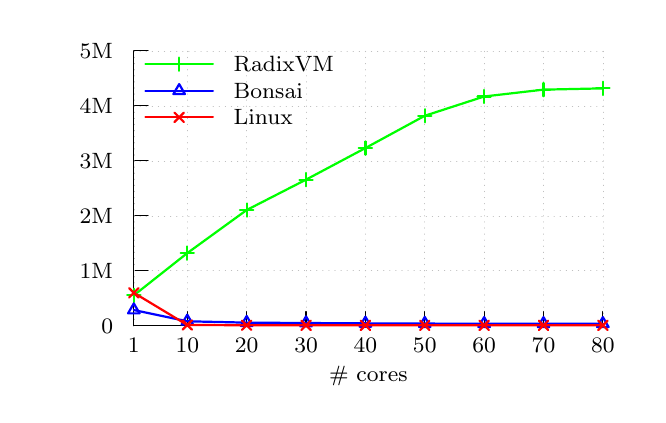
\begin{tikzpicture}[gnuplot]
%% generated with GNUPLOT 5.0p1 (Lua 5.3; terminal rev. 99, script rev. 100)
%% Tue  9 Feb 07:20:54 2016
\tikzset{every node/.append style={font={\fontsize{8.0pt}{9.6pt}\selectfont}}}
\path (0.000,0.000) rectangle (7.747,4.572);
\gpcolor{rgb color={0.753,0.753,0.753}}
\gpsetlinetype{gp lt axes}
\gpsetdashtype{gp dt axes}
\gpsetlinewidth{0.50}
\draw[gp path] (1.348,0.787)--(7.305,0.787);
\gpcolor{color=gp lt color border}
\gpsetlinetype{gp lt border}
\gpsetdashtype{gp dt solid}
\gpsetlinewidth{1.00}
\draw[gp path] (1.348,0.787)--(1.528,0.787);
\node[gp node right] at (1.201,0.787) {   0 };
\gpcolor{rgb color={0.753,0.753,0.753}}
\gpsetlinetype{gp lt axes}
\gpsetdashtype{gp dt axes}
\gpsetlinewidth{0.50}
\draw[gp path] (1.348,1.485)--(7.305,1.485);
\gpcolor{color=gp lt color border}
\gpsetlinetype{gp lt border}
\gpsetdashtype{gp dt solid}
\gpsetlinewidth{1.00}
\draw[gp path] (1.348,1.485)--(1.528,1.485);
\node[gp node right] at (1.201,1.485) {   1M};
\gpcolor{rgb color={0.753,0.753,0.753}}
\gpsetlinetype{gp lt axes}
\gpsetdashtype{gp dt axes}
\gpsetlinewidth{0.50}
\draw[gp path] (1.348,2.183)--(7.305,2.183);
\gpcolor{color=gp lt color border}
\gpsetlinetype{gp lt border}
\gpsetdashtype{gp dt solid}
\gpsetlinewidth{1.00}
\draw[gp path] (1.348,2.183)--(1.528,2.183);
\node[gp node right] at (1.201,2.183) {   2M};
\gpcolor{rgb color={0.753,0.753,0.753}}
\gpsetlinetype{gp lt axes}
\gpsetdashtype{gp dt axes}
\gpsetlinewidth{0.50}
\draw[gp path] (1.348,2.881)--(7.305,2.881);
\gpcolor{color=gp lt color border}
\gpsetlinetype{gp lt border}
\gpsetdashtype{gp dt solid}
\gpsetlinewidth{1.00}
\draw[gp path] (1.348,2.881)--(1.528,2.881);
\node[gp node right] at (1.201,2.881) {   3M};
\gpcolor{rgb color={0.753,0.753,0.753}}
\gpsetlinetype{gp lt axes}
\gpsetdashtype{gp dt axes}
\gpsetlinewidth{0.50}
\draw[gp path] (1.348,3.579)--(7.305,3.579);
\gpcolor{color=gp lt color border}
\gpsetlinetype{gp lt border}
\gpsetdashtype{gp dt solid}
\gpsetlinewidth{1.00}
\draw[gp path] (1.348,3.579)--(1.528,3.579);
\node[gp node right] at (1.201,3.579) {   4M};
\gpcolor{rgb color={0.753,0.753,0.753}}
\gpsetlinetype{gp lt axes}
\gpsetdashtype{gp dt axes}
\gpsetlinewidth{0.50}
\draw[gp path] (1.348,4.277)--(7.305,4.277);
\gpcolor{color=gp lt color border}
\gpsetlinetype{gp lt border}
\gpsetdashtype{gp dt solid}
\gpsetlinewidth{1.00}
\draw[gp path] (1.348,4.277)--(1.528,4.277);
\node[gp node right] at (1.201,4.277) {   5M};
\gpcolor{rgb color={0.753,0.753,0.753}}
\gpsetlinetype{gp lt axes}
\gpsetdashtype{gp dt axes}
\gpsetlinewidth{0.50}
\draw[gp path] (1.348,0.787)--(1.348,4.277);
\gpcolor{color=gp lt color border}
\gpsetlinetype{gp lt border}
\gpsetdashtype{gp dt solid}
\gpsetlinewidth{1.00}
\draw[gp path] (1.348,0.787)--(1.348,0.967);
\node[gp node center] at (1.348,0.541) {$1$};
\gpcolor{rgb color={0.753,0.753,0.753}}
\gpsetlinetype{gp lt axes}
\gpsetdashtype{gp dt axes}
\gpsetlinewidth{0.50}
\draw[gp path] (2.027,0.787)--(2.027,4.277);
\gpcolor{color=gp lt color border}
\gpsetlinetype{gp lt border}
\gpsetdashtype{gp dt solid}
\gpsetlinewidth{1.00}
\draw[gp path] (2.027,0.787)--(2.027,0.967);
\node[gp node center] at (2.027,0.541) {$10$};
\gpcolor{rgb color={0.753,0.753,0.753}}
\gpsetlinetype{gp lt axes}
\gpsetdashtype{gp dt axes}
\gpsetlinewidth{0.50}
\draw[gp path] (2.781,0.787)--(2.781,4.277);
\gpcolor{color=gp lt color border}
\gpsetlinetype{gp lt border}
\gpsetdashtype{gp dt solid}
\gpsetlinewidth{1.00}
\draw[gp path] (2.781,0.787)--(2.781,0.967);
\node[gp node center] at (2.781,0.541) {$20$};
\gpcolor{rgb color={0.753,0.753,0.753}}
\gpsetlinetype{gp lt axes}
\gpsetdashtype{gp dt axes}
\gpsetlinewidth{0.50}
\draw[gp path] (3.535,0.787)--(3.535,4.277);
\gpcolor{color=gp lt color border}
\gpsetlinetype{gp lt border}
\gpsetdashtype{gp dt solid}
\gpsetlinewidth{1.00}
\draw[gp path] (3.535,0.787)--(3.535,0.967);
\node[gp node center] at (3.535,0.541) {$30$};
\gpcolor{rgb color={0.753,0.753,0.753}}
\gpsetlinetype{gp lt axes}
\gpsetdashtype{gp dt axes}
\gpsetlinewidth{0.50}
\draw[gp path] (4.289,0.787)--(4.289,4.277);
\gpcolor{color=gp lt color border}
\gpsetlinetype{gp lt border}
\gpsetdashtype{gp dt solid}
\gpsetlinewidth{1.00}
\draw[gp path] (4.289,0.787)--(4.289,0.967);
\node[gp node center] at (4.289,0.541) {$40$};
\gpcolor{rgb color={0.753,0.753,0.753}}
\gpsetlinetype{gp lt axes}
\gpsetdashtype{gp dt axes}
\gpsetlinewidth{0.50}
\draw[gp path] (5.043,0.787)--(5.043,4.277);
\gpcolor{color=gp lt color border}
\gpsetlinetype{gp lt border}
\gpsetdashtype{gp dt solid}
\gpsetlinewidth{1.00}
\draw[gp path] (5.043,0.787)--(5.043,0.967);
\node[gp node center] at (5.043,0.541) {$50$};
\gpcolor{rgb color={0.753,0.753,0.753}}
\gpsetlinetype{gp lt axes}
\gpsetdashtype{gp dt axes}
\gpsetlinewidth{0.50}
\draw[gp path] (5.797,0.787)--(5.797,4.277);
\gpcolor{color=gp lt color border}
\gpsetlinetype{gp lt border}
\gpsetdashtype{gp dt solid}
\gpsetlinewidth{1.00}
\draw[gp path] (5.797,0.787)--(5.797,0.967);
\node[gp node center] at (5.797,0.541) {$60$};
\gpcolor{rgb color={0.753,0.753,0.753}}
\gpsetlinetype{gp lt axes}
\gpsetdashtype{gp dt axes}
\gpsetlinewidth{0.50}
\draw[gp path] (6.551,0.787)--(6.551,4.277);
\gpcolor{color=gp lt color border}
\gpsetlinetype{gp lt border}
\gpsetdashtype{gp dt solid}
\gpsetlinewidth{1.00}
\draw[gp path] (6.551,0.787)--(6.551,0.967);
\node[gp node center] at (6.551,0.541) {$70$};
\gpcolor{rgb color={0.753,0.753,0.753}}
\gpsetlinetype{gp lt axes}
\gpsetdashtype{gp dt axes}
\gpsetlinewidth{0.50}
\draw[gp path] (7.305,0.787)--(7.305,4.277);
\gpcolor{color=gp lt color border}
\gpsetlinetype{gp lt border}
\gpsetdashtype{gp dt solid}
\gpsetlinewidth{1.00}
\draw[gp path] (7.305,0.787)--(7.305,0.967);
\node[gp node center] at (7.305,0.541) {$80$};
\gpsetlinetype{gp lt axes}
\gpsetdashtype{gp dt axes}
\draw[gp path] (1.348,0.787)--(7.305,0.787);
\gpsetlinetype{gp lt border}
\gpsetdashtype{gp dt solid}
\draw[gp path] (1.348,4.277)--(1.348,0.787)--(7.305,0.787);
\node[gp node center,rotate=-270] at (0.196,2.532) {~};
\node[gp node center] at (4.326,0.172) {\# cores};
%%%%%%%%%%%%%%%%%%%%%%%%%%%%%%%%%%%%%%%%%%%%%%%%%%
% SDP: Add legend
\node[gp node left] at (2.500,4.108) {\vm}; % AL
\gpcolor{color=gp lt color 1}
\gpsetlinewidth{2.00}
\draw[gp path] (1.495,4.108)--(2.353,4.108); % AL
\draw[gp path] (1.348,1.172)--(2.027,1.709)--(2.781,2.256)--(3.535,2.642)--(4.289,3.043)%
  --(5.043,3.453)--(5.797,3.698)--(6.551,3.785)--(7.305,3.801);
\gpsetpointsize{6.00}
\gppoint{gp mark 1}{(1.348,1.172)}
\gppoint{gp mark 1}{(2.027,1.709)}
\gppoint{gp mark 1}{(2.781,2.256)}
\gppoint{gp mark 1}{(3.535,2.642)}
\gppoint{gp mark 1}{(4.289,3.043)}
\gppoint{gp mark 1}{(5.043,3.453)}
\gppoint{gp mark 1}{(5.797,3.698)}
\gppoint{gp mark 1}{(6.551,3.785)}
\gppoint{gp mark 1}{(7.305,3.801)}
\gppoint{gp mark 1}{(1.924,4.108)} % AL
%%%%%%%%%%%%%%%%%%%%%%%%%%%%%%%%%%%%%%%%%%%%%%%%%%%%%%%%%%%%%%%%%%%%%%
\gpcolor{color=gp lt color border} % AL
\node[gp node left] at (2.500,3.771) {Bonsai}; % AL
\gpcolor{color=gp lt color 2}
\draw[gp path] (1.495,3.771)--(2.353,3.771); % AL
\draw[gp path] (1.348,0.986)--(2.027,0.843)--(2.781,0.826)--(3.535,0.821)--(4.289,0.817)%
  --(5.043,0.814)--(5.797,0.812)--(6.551,0.812)--(7.305,0.812);
\gppoint{gp mark 8}{(1.348,0.986)}
\gppoint{gp mark 8}{(2.027,0.843)}
\gppoint{gp mark 8}{(2.781,0.826)}
\gppoint{gp mark 8}{(3.535,0.821)}
\gppoint{gp mark 8}{(4.289,0.817)}
\gppoint{gp mark 8}{(5.043,0.814)}
\gppoint{gp mark 8}{(5.797,0.812)}
\gppoint{gp mark 8}{(6.551,0.812)}
\gppoint{gp mark 8}{(7.305,0.812)}
\gppoint{gp mark 8}{(1.924,3.771)} % AL
%%%%%%%%%%%%%%%%%%%%%%%%%%%%%%%%%%%%%%%%%%%%%%%%%%%%%%%%%%%%%%%%%%%%%%
\gpcolor{color=gp lt color border} % AL
\node[gp node left] at (2.500,3.434) {Linux}; % AL
\gpcolor{color=gp lt color 0}
\draw[gp path] (1.495,3.434)--(2.353,3.434); % AL
\draw[gp path] (1.348,1.205)--(2.027,0.796)--(2.781,0.793)--(3.535,0.792)--(4.289,0.792)%
  --(5.043,0.792)--(5.797,0.792)--(6.551,0.792)--(7.305,0.792);
\gppoint{gp mark 2}{(1.348,1.205)}
\gppoint{gp mark 2}{(2.027,0.796)}
\gppoint{gp mark 2}{(2.781,0.793)}
\gppoint{gp mark 2}{(3.535,0.792)}
\gppoint{gp mark 2}{(4.289,0.792)}
\gppoint{gp mark 2}{(5.043,0.792)}
\gppoint{gp mark 2}{(5.797,0.792)}
\gppoint{gp mark 2}{(6.551,0.792)}
\gppoint{gp mark 2}{(7.305,0.792)}
\gppoint{gp mark 2}{(1.924,3.434)} % AL
%% coordinates of the plot area
\gpdefrectangularnode{gp plot 1}{\pgfpoint{1.348cm}{0.787cm}}{\pgfpoint{7.305cm}{4.277cm}}
\end{tikzpicture}
%% gnuplot variables

    \end{column}
  \end{columns}
\end{frame}

\begin{frame}{Microbenchmark: Global}
  \begin{columns}[T]
    \begin{column}{0.5\textwidth}
      \bi
    \item Each thread \texttt{mmap} a 64KB region within a large region of memory
      \pause
    \item All threads access all pages in random order
      \ei
    \end{column}
    \begin{column}{0.5\textwidth}
      \pause
      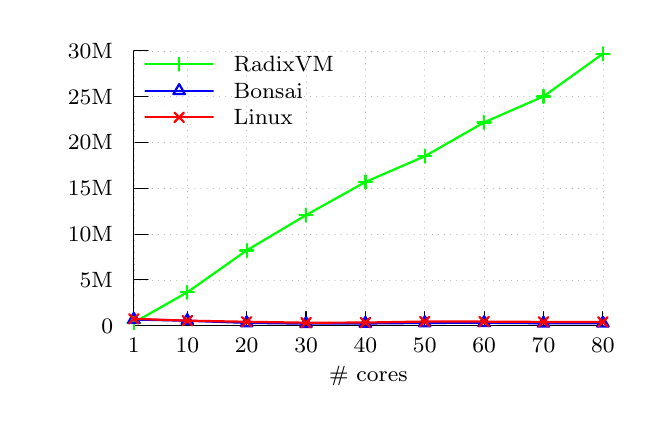
\begin{tikzpicture}[gnuplot]
%% generated with GNUPLOT 5.0p1 (Lua 5.3; terminal rev. 99, script rev. 100)
%% Tue  9 Feb 07:20:52 2016
\tikzset{every node/.append style={font={\fontsize{8.0pt}{9.6pt}\selectfont}}}
\path (0.000,0.000) rectangle (7.747,4.572);
\gpcolor{rgb color={0.753,0.753,0.753}}
\gpsetlinetype{gp lt axes}
\gpsetdashtype{gp dt axes}
\gpsetlinewidth{0.50}
\draw[gp path] (1.348,0.787)--(7.305,0.787);
\gpcolor{color=gp lt color border}
\gpsetlinetype{gp lt border}
\gpsetdashtype{gp dt solid}
\gpsetlinewidth{1.00}
\draw[gp path] (1.348,0.787)--(1.528,0.787);
\node[gp node right] at (1.201,0.787) {  0 };
\gpcolor{rgb color={0.753,0.753,0.753}}
\gpsetlinetype{gp lt axes}
\gpsetdashtype{gp dt axes}
\gpsetlinewidth{0.50}
\draw[gp path] (1.348,1.369)--(7.305,1.369);
\gpcolor{color=gp lt color border}
\gpsetlinetype{gp lt border}
\gpsetdashtype{gp dt solid}
\gpsetlinewidth{1.00}
\draw[gp path] (1.348,1.369)--(1.528,1.369);
\node[gp node right] at (1.201,1.369) {  5M};
\gpcolor{rgb color={0.753,0.753,0.753}}
\gpsetlinetype{gp lt axes}
\gpsetdashtype{gp dt axes}
\gpsetlinewidth{0.50}
\draw[gp path] (1.348,1.950)--(7.305,1.950);
\gpcolor{color=gp lt color border}
\gpsetlinetype{gp lt border}
\gpsetdashtype{gp dt solid}
\gpsetlinewidth{1.00}
\draw[gp path] (1.348,1.950)--(1.528,1.950);
\node[gp node right] at (1.201,1.950) {  10M};
\gpcolor{rgb color={0.753,0.753,0.753}}
\gpsetlinetype{gp lt axes}
\gpsetdashtype{gp dt axes}
\gpsetlinewidth{0.50}
\draw[gp path] (1.348,2.532)--(7.305,2.532);
\gpcolor{color=gp lt color border}
\gpsetlinetype{gp lt border}
\gpsetdashtype{gp dt solid}
\gpsetlinewidth{1.00}
\draw[gp path] (1.348,2.532)--(1.528,2.532);
\node[gp node right] at (1.201,2.532) {  15M};
\gpcolor{rgb color={0.753,0.753,0.753}}
\gpsetlinetype{gp lt axes}
\gpsetdashtype{gp dt axes}
\gpsetlinewidth{0.50}
\draw[gp path] (1.348,3.114)--(7.305,3.114);
\gpcolor{color=gp lt color border}
\gpsetlinetype{gp lt border}
\gpsetdashtype{gp dt solid}
\gpsetlinewidth{1.00}
\draw[gp path] (1.348,3.114)--(1.528,3.114);
\node[gp node right] at (1.201,3.114) {  20M};
\gpcolor{rgb color={0.753,0.753,0.753}}
\gpsetlinetype{gp lt axes}
\gpsetdashtype{gp dt axes}
\gpsetlinewidth{0.50}
\draw[gp path] (1.348,3.695)--(7.305,3.695);
\gpcolor{color=gp lt color border}
\gpsetlinetype{gp lt border}
\gpsetdashtype{gp dt solid}
\gpsetlinewidth{1.00}
\draw[gp path] (1.348,3.695)--(1.528,3.695);
\node[gp node right] at (1.201,3.695) {  25M};
\gpcolor{rgb color={0.753,0.753,0.753}}
\gpsetlinetype{gp lt axes}
\gpsetdashtype{gp dt axes}
\gpsetlinewidth{0.50}
\draw[gp path] (1.348,4.277)--(7.305,4.277);
\gpcolor{color=gp lt color border}
\gpsetlinetype{gp lt border}
\gpsetdashtype{gp dt solid}
\gpsetlinewidth{1.00}
\draw[gp path] (1.348,4.277)--(1.528,4.277);
\node[gp node right] at (1.201,4.277) {  30M};
\gpcolor{rgb color={0.753,0.753,0.753}}
\gpsetlinetype{gp lt axes}
\gpsetdashtype{gp dt axes}
\gpsetlinewidth{0.50}
\draw[gp path] (1.348,0.787)--(1.348,4.277);
\gpcolor{color=gp lt color border}
\gpsetlinetype{gp lt border}
\gpsetdashtype{gp dt solid}
\gpsetlinewidth{1.00}
\draw[gp path] (1.348,0.787)--(1.348,0.967);
\node[gp node center] at (1.348,0.541) {$1$};
\gpcolor{rgb color={0.753,0.753,0.753}}
\gpsetlinetype{gp lt axes}
\gpsetdashtype{gp dt axes}
\gpsetlinewidth{0.50}
\draw[gp path] (2.027,0.787)--(2.027,4.277);
\gpcolor{color=gp lt color border}
\gpsetlinetype{gp lt border}
\gpsetdashtype{gp dt solid}
\gpsetlinewidth{1.00}
\draw[gp path] (2.027,0.787)--(2.027,0.967);
\node[gp node center] at (2.027,0.541) {$10$};
\gpcolor{rgb color={0.753,0.753,0.753}}
\gpsetlinetype{gp lt axes}
\gpsetdashtype{gp dt axes}
\gpsetlinewidth{0.50}
\draw[gp path] (2.781,0.787)--(2.781,4.277);
\gpcolor{color=gp lt color border}
\gpsetlinetype{gp lt border}
\gpsetdashtype{gp dt solid}
\gpsetlinewidth{1.00}
\draw[gp path] (2.781,0.787)--(2.781,0.967);
\node[gp node center] at (2.781,0.541) {$20$};
\gpcolor{rgb color={0.753,0.753,0.753}}
\gpsetlinetype{gp lt axes}
\gpsetdashtype{gp dt axes}
\gpsetlinewidth{0.50}
\draw[gp path] (3.535,0.787)--(3.535,4.277);
\gpcolor{color=gp lt color border}
\gpsetlinetype{gp lt border}
\gpsetdashtype{gp dt solid}
\gpsetlinewidth{1.00}
\draw[gp path] (3.535,0.787)--(3.535,0.967);
\node[gp node center] at (3.535,0.541) {$30$};
\gpcolor{rgb color={0.753,0.753,0.753}}
\gpsetlinetype{gp lt axes}
\gpsetdashtype{gp dt axes}
\gpsetlinewidth{0.50}
\draw[gp path] (4.289,0.787)--(4.289,4.277);
\gpcolor{color=gp lt color border}
\gpsetlinetype{gp lt border}
\gpsetdashtype{gp dt solid}
\gpsetlinewidth{1.00}
\draw[gp path] (4.289,0.787)--(4.289,0.967);
\node[gp node center] at (4.289,0.541) {$40$};
\gpcolor{rgb color={0.753,0.753,0.753}}
\gpsetlinetype{gp lt axes}
\gpsetdashtype{gp dt axes}
\gpsetlinewidth{0.50}
\draw[gp path] (5.043,0.787)--(5.043,4.277);
\gpcolor{color=gp lt color border}
\gpsetlinetype{gp lt border}
\gpsetdashtype{gp dt solid}
\gpsetlinewidth{1.00}
\draw[gp path] (5.043,0.787)--(5.043,0.967);
\node[gp node center] at (5.043,0.541) {$50$};
\gpcolor{rgb color={0.753,0.753,0.753}}
\gpsetlinetype{gp lt axes}
\gpsetdashtype{gp dt axes}
\gpsetlinewidth{0.50}
\draw[gp path] (5.797,0.787)--(5.797,4.277);
\gpcolor{color=gp lt color border}
\gpsetlinetype{gp lt border}
\gpsetdashtype{gp dt solid}
\gpsetlinewidth{1.00}
\draw[gp path] (5.797,0.787)--(5.797,0.967);
\node[gp node center] at (5.797,0.541) {$60$};
\gpcolor{rgb color={0.753,0.753,0.753}}
\gpsetlinetype{gp lt axes}
\gpsetdashtype{gp dt axes}
\gpsetlinewidth{0.50}
\draw[gp path] (6.551,0.787)--(6.551,4.277);
\gpcolor{color=gp lt color border}
\gpsetlinetype{gp lt border}
\gpsetdashtype{gp dt solid}
\gpsetlinewidth{1.00}
\draw[gp path] (6.551,0.787)--(6.551,0.967);
\node[gp node center] at (6.551,0.541) {$70$};
\gpcolor{rgb color={0.753,0.753,0.753}}
\gpsetlinetype{gp lt axes}
\gpsetdashtype{gp dt axes}
\gpsetlinewidth{0.50}
\draw[gp path] (7.305,0.787)--(7.305,4.277);
\gpcolor{color=gp lt color border}
\gpsetlinetype{gp lt border}
\gpsetdashtype{gp dt solid}
\gpsetlinewidth{1.00}
\draw[gp path] (7.305,0.787)--(7.305,0.967);
\node[gp node center] at (7.305,0.541) {$80$};
\gpsetlinetype{gp lt axes}
\gpsetdashtype{gp dt axes}
\draw[gp path] (1.348,0.787)--(7.305,0.787);
\gpsetlinetype{gp lt border}
\gpsetdashtype{gp dt solid}
\draw[gp path] (1.348,4.277)--(1.348,0.787)--(7.305,0.787);
\node[gp node center,rotate=-270] at (0.196,2.532) {~};
\node[gp node center] at (4.326,0.172) {\# cores};
%%%%%%%%%%%%%%%%%%%%%%%%%%%%%%%%%%%%%%%%%%%%%%%%%%
% SDP: Add legend
\node[gp node left] at (2.500,4.108) {\vm}; % AL
\gpcolor{color=gp lt color 1}
\gpsetlinewidth{2.00}
\draw[gp path] (1.495,4.108)--(2.353,4.108); % AL
\draw[gp path] (1.348,0.826)--(2.027,1.211)--(2.781,1.743)--(3.535,2.191)--(4.289,2.612)%
  --(5.043,2.939)--(5.797,3.369)--(6.551,3.699)--(7.305,4.240);
\gpsetpointsize{6.00}
\gppoint{gp mark 1}{(1.348,0.826)}
\gppoint{gp mark 1}{(2.027,1.211)}
\gppoint{gp mark 1}{(2.781,1.743)}
\gppoint{gp mark 1}{(3.535,2.191)}
\gppoint{gp mark 1}{(4.289,2.612)}
\gppoint{gp mark 1}{(5.043,2.939)}
\gppoint{gp mark 1}{(5.797,3.369)}
\gppoint{gp mark 1}{(6.551,3.699)}
\gppoint{gp mark 1}{(7.305,4.240)}
\gppoint{gp mark 1}{(1.924,4.108)} % AL
%%%%%%%%%%%%%%%%%%%%%%%%%%%%%%%%%%%%%%%%%%%%%%%%%%%%%%%%%%%%%%%%%%%%%%
\gpcolor{color=gp lt color border} % AL
\node[gp node left] at (2.500,3.771) {Bonsai}; % AL
\gpcolor{color=gp lt color 2}
\draw[gp path] (1.495,3.771)--(2.353,3.771); % AL
\draw[gp path] (1.348,0.866)--(2.027,0.850)--(2.781,0.823)--(3.535,0.813)--(4.289,0.815)%
  --(5.043,0.822)--(5.797,0.824)--(6.551,0.818)--(7.305,0.818);
\gppoint{gp mark 8}{(1.348,0.866)}
\gppoint{gp mark 8}{(2.027,0.850)}
\gppoint{gp mark 8}{(2.781,0.823)}
\gppoint{gp mark 8}{(3.535,0.813)}
\gppoint{gp mark 8}{(4.289,0.815)}
\gppoint{gp mark 8}{(5.043,0.822)}
\gppoint{gp mark 8}{(5.797,0.824)}
\gppoint{gp mark 8}{(6.551,0.818)}
\gppoint{gp mark 8}{(7.305,0.818)}
\gppoint{gp mark 8}{(1.924,3.771)} % AL
%%%%%%%%%%%%%%%%%%%%%%%%%%%%%%%%%%%%%%%%%%%%%%%%%%%%%%%%%%%%%%%%%%%%%%
\gpcolor{color=gp lt color border} % AL
\node[gp node left] at (2.500,3.434) {Linux}; % AL
\gpcolor{color=gp lt color 0}
\draw[gp path] (1.495,3.434)--(2.353,3.434); % AL
\draw[gp path] (1.348,0.875)--(2.027,0.851)--(2.781,0.837)--(3.535,0.825)--(4.289,0.827)%
  --(5.043,0.840)--(5.797,0.839)--(6.551,0.835)--(7.305,0.835);
\gppoint{gp mark 2}{(1.348,0.875)}
\gppoint{gp mark 2}{(2.027,0.851)}
\gppoint{gp mark 2}{(2.781,0.837)}
\gppoint{gp mark 2}{(3.535,0.825)}
\gppoint{gp mark 2}{(4.289,0.827)}
\gppoint{gp mark 2}{(5.043,0.840)}
\gppoint{gp mark 2}{(5.797,0.839)}
\gppoint{gp mark 2}{(6.551,0.835)}
\gppoint{gp mark 2}{(7.305,0.835)}
\gppoint{gp mark 2}{(1.924,3.434)} % AL
%% coordinates of the plot area
\gpdefrectangularnode{gp plot 1}{\pgfpoint{1.348cm}{0.787cm}}{\pgfpoint{7.305cm}{4.277cm}}
\end{tikzpicture}
%% gnuplot variables

    \end{column}
  \end{columns}
\end{frame}

\begin{frame}{Question}
  \begin{columns}[T]
    \begin{column}{0.3\textwidth}
    \end{column}
    \begin{column}{0.4\textwidth}
      Do we really need all 3 pieces?
      \bi
    \item Radix trees
    \item Refcache
    \item Targeted TLB shootdown
      \ei
    \end{column}
    \begin{column}{0.3\textwidth}
    \end{column}
  \end{columns}
\end{frame}

\begin{frame}{Question: Do we need radix trees?}
  \begin{columns}[T]
    \begin{column}{0.5\textwidth}
      \begin{center}
        Skip lists\\
        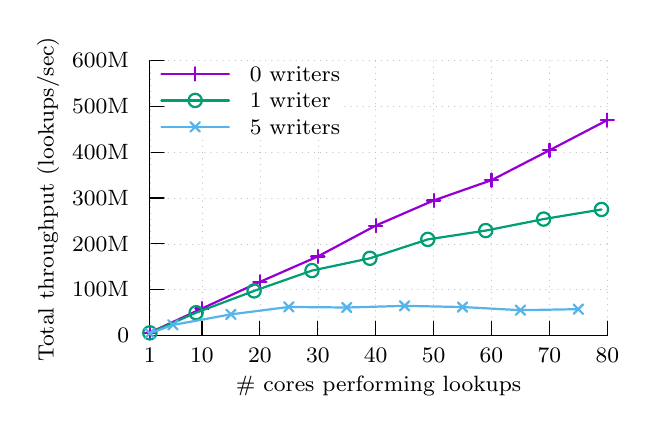
\begin{tikzpicture}[gnuplot]
%% generated with GNUPLOT 5.0p1 (Lua 5.3; terminal rev. 99, script rev. 100)
%% Tue  9 Feb 07:20:54 2016
\tikzset{every node/.append style={font={\fontsize{8.0pt}{9.6pt}\selectfont}}}
\path (0.000,0.000) rectangle (7.747,4.572);
\gpcolor{rgb color={0.753,0.753,0.753}}
\gpsetlinetype{gp lt axes}
\gpsetdashtype{gp dt axes}
\gpsetlinewidth{0.50}
\draw[gp path] (1.495,0.787)--(7.305,0.787);
\gpcolor{color=gp lt color border}
\gpsetlinetype{gp lt border}
\gpsetdashtype{gp dt solid}
\gpsetlinewidth{1.00}
\draw[gp path] (1.495,0.787)--(1.675,0.787);
\node[gp node right] at (1.348,0.787) {  0 };
\gpcolor{rgb color={0.753,0.753,0.753}}
\gpsetlinetype{gp lt axes}
\gpsetdashtype{gp dt axes}
\gpsetlinewidth{0.50}
\draw[gp path] (1.495,1.369)--(7.305,1.369);
\gpcolor{color=gp lt color border}
\gpsetlinetype{gp lt border}
\gpsetdashtype{gp dt solid}
\gpsetlinewidth{1.00}
\draw[gp path] (1.495,1.369)--(1.675,1.369);
\node[gp node right] at (1.348,1.369) {  100M};
\gpcolor{rgb color={0.753,0.753,0.753}}
\gpsetlinetype{gp lt axes}
\gpsetdashtype{gp dt axes}
\gpsetlinewidth{0.50}
\draw[gp path] (1.495,1.950)--(7.305,1.950);
\gpcolor{color=gp lt color border}
\gpsetlinetype{gp lt border}
\gpsetdashtype{gp dt solid}
\gpsetlinewidth{1.00}
\draw[gp path] (1.495,1.950)--(1.675,1.950);
\node[gp node right] at (1.348,1.950) {  200M};
\gpcolor{rgb color={0.753,0.753,0.753}}
\gpsetlinetype{gp lt axes}
\gpsetdashtype{gp dt axes}
\gpsetlinewidth{0.50}
\draw[gp path] (1.495,2.532)--(7.305,2.532);
\gpcolor{color=gp lt color border}
\gpsetlinetype{gp lt border}
\gpsetdashtype{gp dt solid}
\gpsetlinewidth{1.00}
\draw[gp path] (1.495,2.532)--(1.675,2.532);
\node[gp node right] at (1.348,2.532) {  300M};
\gpcolor{rgb color={0.753,0.753,0.753}}
\gpsetlinetype{gp lt axes}
\gpsetdashtype{gp dt axes}
\gpsetlinewidth{0.50}
\draw[gp path] (1.495,3.114)--(7.305,3.114);
\gpcolor{color=gp lt color border}
\gpsetlinetype{gp lt border}
\gpsetdashtype{gp dt solid}
\gpsetlinewidth{1.00}
\draw[gp path] (1.495,3.114)--(1.675,3.114);
\node[gp node right] at (1.348,3.114) {  400M};
\gpcolor{rgb color={0.753,0.753,0.753}}
\gpsetlinetype{gp lt axes}
\gpsetdashtype{gp dt axes}
\gpsetlinewidth{0.50}
\draw[gp path] (3.970,3.695)--(7.305,3.695);
\gpcolor{color=gp lt color border}
\gpsetlinetype{gp lt border}
\gpsetdashtype{gp dt solid}
\gpsetlinewidth{1.00}
\draw[gp path] (1.495,3.695)--(1.675,3.695);
\node[gp node right] at (1.348,3.695) {  500M};
\gpcolor{rgb color={0.753,0.753,0.753}}
\gpsetlinetype{gp lt axes}
\gpsetdashtype{gp dt axes}
\gpsetlinewidth{0.50}
\draw[gp path] (1.495,4.277)--(7.305,4.277);
\gpcolor{color=gp lt color border}
\gpsetlinetype{gp lt border}
\gpsetdashtype{gp dt solid}
\gpsetlinewidth{1.00}
\draw[gp path] (1.495,4.277)--(1.675,4.277);
\node[gp node right] at (1.348,4.277) {  600M};
\gpcolor{rgb color={0.753,0.753,0.753}}
\gpsetlinetype{gp lt axes}
\gpsetdashtype{gp dt axes}
\gpsetlinewidth{0.50}
\draw[gp path] (1.495,0.787)--(1.495,4.277);
\gpcolor{color=gp lt color border}
\gpsetlinetype{gp lt border}
\gpsetdashtype{gp dt solid}
\gpsetlinewidth{1.00}
\draw[gp path] (1.495,0.787)--(1.495,0.967);
\node[gp node center] at (1.495,0.541) {$1$};
\gpcolor{rgb color={0.753,0.753,0.753}}
\gpsetlinetype{gp lt axes}
\gpsetdashtype{gp dt axes}
\gpsetlinewidth{0.50}
\draw[gp path] (2.157,0.787)--(2.157,3.266);
\gpcolor{color=gp lt color border}
\gpsetlinetype{gp lt border}
\gpsetdashtype{gp dt solid}
\gpsetlinewidth{1.00}
\draw[gp path] (2.157,0.787)--(2.157,0.967);
\node[gp node center] at (2.157,0.541) {$10$};
\gpcolor{rgb color={0.753,0.753,0.753}}
\gpsetlinetype{gp lt axes}
\gpsetdashtype{gp dt axes}
\gpsetlinewidth{0.50}
\draw[gp path] (2.892,0.787)--(2.892,3.266);
\gpcolor{color=gp lt color border}
\gpsetlinetype{gp lt border}
\gpsetdashtype{gp dt solid}
\gpsetlinewidth{1.00}
\draw[gp path] (2.892,0.787)--(2.892,0.967);
\node[gp node center] at (2.892,0.541) {$20$};
\gpcolor{rgb color={0.753,0.753,0.753}}
\gpsetlinetype{gp lt axes}
\gpsetdashtype{gp dt axes}
\gpsetlinewidth{0.50}
\draw[gp path] (3.628,0.787)--(3.628,3.266);
\gpcolor{color=gp lt color border}
\gpsetlinetype{gp lt border}
\gpsetdashtype{gp dt solid}
\gpsetlinewidth{1.00}
\draw[gp path] (3.628,0.787)--(3.628,0.967);
\node[gp node center] at (3.628,0.541) {$30$};
\gpcolor{rgb color={0.753,0.753,0.753}}
\gpsetlinetype{gp lt axes}
\gpsetdashtype{gp dt axes}
\gpsetlinewidth{0.50}
\draw[gp path] (4.363,0.787)--(4.363,4.277);
\gpcolor{color=gp lt color border}
\gpsetlinetype{gp lt border}
\gpsetdashtype{gp dt solid}
\gpsetlinewidth{1.00}
\draw[gp path] (4.363,0.787)--(4.363,0.967);
\node[gp node center] at (4.363,0.541) {$40$};
\gpcolor{rgb color={0.753,0.753,0.753}}
\gpsetlinetype{gp lt axes}
\gpsetdashtype{gp dt axes}
\gpsetlinewidth{0.50}
\draw[gp path] (5.099,0.787)--(5.099,4.277);
\gpcolor{color=gp lt color border}
\gpsetlinetype{gp lt border}
\gpsetdashtype{gp dt solid}
\gpsetlinewidth{1.00}
\draw[gp path] (5.099,0.787)--(5.099,0.967);
\node[gp node center] at (5.099,0.541) {$50$};
\gpcolor{rgb color={0.753,0.753,0.753}}
\gpsetlinetype{gp lt axes}
\gpsetdashtype{gp dt axes}
\gpsetlinewidth{0.50}
\draw[gp path] (5.834,0.787)--(5.834,4.277);
\gpcolor{color=gp lt color border}
\gpsetlinetype{gp lt border}
\gpsetdashtype{gp dt solid}
\gpsetlinewidth{1.00}
\draw[gp path] (5.834,0.787)--(5.834,0.967);
\node[gp node center] at (5.834,0.541) {$60$};
\gpcolor{rgb color={0.753,0.753,0.753}}
\gpsetlinetype{gp lt axes}
\gpsetdashtype{gp dt axes}
\gpsetlinewidth{0.50}
\draw[gp path] (6.570,0.787)--(6.570,4.277);
\gpcolor{color=gp lt color border}
\gpsetlinetype{gp lt border}
\gpsetdashtype{gp dt solid}
\gpsetlinewidth{1.00}
\draw[gp path] (6.570,0.787)--(6.570,0.967);
\node[gp node center] at (6.570,0.541) {$70$};
\gpcolor{rgb color={0.753,0.753,0.753}}
\gpsetlinetype{gp lt axes}
\gpsetdashtype{gp dt axes}
\gpsetlinewidth{0.50}
\draw[gp path] (7.305,0.787)--(7.305,4.277);
\gpcolor{color=gp lt color border}
\gpsetlinetype{gp lt border}
\gpsetdashtype{gp dt solid}
\gpsetlinewidth{1.00}
\draw[gp path] (7.305,0.787)--(7.305,0.967);
\node[gp node center] at (7.305,0.541) {$80$};
\gpsetlinetype{gp lt axes}
\gpsetdashtype{gp dt axes}
\draw[gp path] (1.495,0.787)--(7.305,0.787);
\gpsetlinetype{gp lt border}
\gpsetdashtype{gp dt solid}
\draw[gp path] (1.495,4.277)--(1.495,0.787)--(7.305,0.787);
\node[gp node center,rotate=-270] at (0.196,2.532) {Total throughput (lookups/sec)};
\node[gp node center] at (4.400,0.172) {\# cores performing lookups};
\node[gp node left] at (2.647,4.108) {0 writers};
\gpcolor{rgb color={0.580,0.000,0.827}}
\gpsetlinewidth{2.00}
\draw[gp path] (1.642,4.108)--(2.500,4.108);
\draw[gp path] (1.495,0.822)--(2.157,1.128)--(2.892,1.466)--(3.628,1.789)--(4.363,2.181)%
  --(5.099,2.500)--(5.834,2.758)--(6.570,3.138)--(7.305,3.521);
\gpsetpointsize{6.00}
\gppoint{gp mark 1}{(1.495,0.822)}
\gppoint{gp mark 1}{(2.157,1.128)}
\gppoint{gp mark 1}{(2.892,1.466)}
\gppoint{gp mark 1}{(3.628,1.789)}
\gppoint{gp mark 1}{(4.363,2.181)}
\gppoint{gp mark 1}{(5.099,2.500)}
\gppoint{gp mark 1}{(5.834,2.758)}
\gppoint{gp mark 1}{(6.570,3.138)}
\gppoint{gp mark 1}{(7.305,3.521)}
\gppoint{gp mark 1}{(2.071,4.108)}
\gpcolor{color=gp lt color border}
\node[gp node left] at (2.647,3.771) {1 writer};
\gpcolor{rgb color={0.000,0.620,0.451}}
\draw[gp path] (1.642,3.771)--(2.500,3.771);
\draw[gp path] (1.495,0.819)--(2.083,1.075)--(2.819,1.352)--(3.554,1.610)--(4.290,1.766)%
  --(5.025,2.006)--(5.761,2.118)--(6.496,2.264)--(7.231,2.386);
\gppoint{gp mark 6}{(1.495,0.819)}
\gppoint{gp mark 6}{(2.083,1.075)}
\gppoint{gp mark 6}{(2.819,1.352)}
\gppoint{gp mark 6}{(3.554,1.610)}
\gppoint{gp mark 6}{(4.290,1.766)}
\gppoint{gp mark 6}{(5.025,2.006)}
\gppoint{gp mark 6}{(5.761,2.118)}
\gppoint{gp mark 6}{(6.496,2.264)}
\gppoint{gp mark 6}{(7.231,2.386)}
\gppoint{gp mark 6}{(2.071,3.771)}
\gpcolor{color=gp lt color border}
\node[gp node left] at (2.647,3.434) {5 writers};
\gpcolor{rgb color={0.337,0.706,0.914}}
\draw[gp path] (1.642,3.434)--(2.500,3.434);
\draw[gp path] (1.495,0.813)--(1.789,0.920)--(2.525,1.054)--(3.260,1.148)--(3.996,1.141)%
  --(4.731,1.162)--(5.466,1.147)--(6.202,1.107)--(6.937,1.120);
\gppoint{gp mark 2}{(1.495,0.813)}
\gppoint{gp mark 2}{(1.789,0.920)}
\gppoint{gp mark 2}{(2.525,1.054)}
\gppoint{gp mark 2}{(3.260,1.148)}
\gppoint{gp mark 2}{(3.996,1.141)}
\gppoint{gp mark 2}{(4.731,1.162)}
\gppoint{gp mark 2}{(5.466,1.147)}
\gppoint{gp mark 2}{(6.202,1.107)}
\gppoint{gp mark 2}{(6.937,1.120)}
\gppoint{gp mark 2}{(2.071,3.434)}
%% coordinates of the plot area
\gpdefrectangularnode{gp plot 1}{\pgfpoint{1.495cm}{0.787cm}}{\pgfpoint{7.305cm}{4.277cm}}
\end{tikzpicture}
%% gnuplot variables

      \end{center}
    \end{column}
    \begin{column}{0.5\textwidth}
      \begin{center}
        \pause
        Radix trees\\
        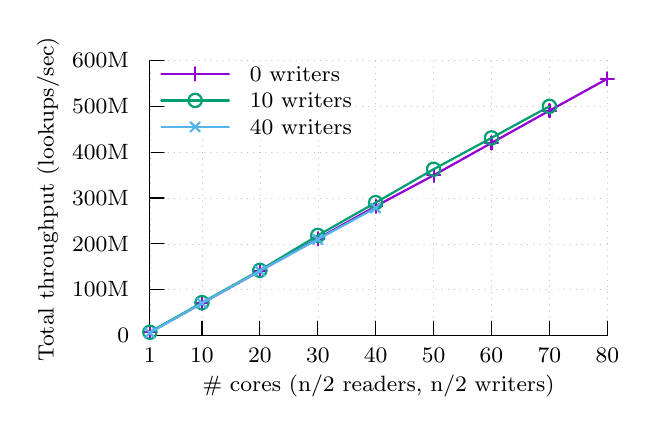
\begin{tikzpicture}[gnuplot]
%% generated with GNUPLOT 5.0p1 (Lua 5.3; terminal rev. 99, script rev. 100)
%% Tue  9 Feb 07:20:54 2016
\tikzset{every node/.append style={font={\fontsize{8.0pt}{9.6pt}\selectfont}}}
\path (0.000,0.000) rectangle (7.747,4.572);
\gpcolor{rgb color={0.753,0.753,0.753}}
\gpsetlinetype{gp lt axes}
\gpsetdashtype{gp dt axes}
\gpsetlinewidth{0.50}
\draw[gp path] (1.495,0.787)--(7.305,0.787);
\gpcolor{color=gp lt color border}
\gpsetlinetype{gp lt border}
\gpsetdashtype{gp dt solid}
\gpsetlinewidth{1.00}
\draw[gp path] (1.495,0.787)--(1.675,0.787);
\node[gp node right] at (1.348,0.787) {  0 };
\gpcolor{rgb color={0.753,0.753,0.753}}
\gpsetlinetype{gp lt axes}
\gpsetdashtype{gp dt axes}
\gpsetlinewidth{0.50}
\draw[gp path] (1.495,1.369)--(7.305,1.369);
\gpcolor{color=gp lt color border}
\gpsetlinetype{gp lt border}
\gpsetdashtype{gp dt solid}
\gpsetlinewidth{1.00}
\draw[gp path] (1.495,1.369)--(1.675,1.369);
\node[gp node right] at (1.348,1.369) {  100M};
\gpcolor{rgb color={0.753,0.753,0.753}}
\gpsetlinetype{gp lt axes}
\gpsetdashtype{gp dt axes}
\gpsetlinewidth{0.50}
\draw[gp path] (1.495,1.950)--(7.305,1.950);
\gpcolor{color=gp lt color border}
\gpsetlinetype{gp lt border}
\gpsetdashtype{gp dt solid}
\gpsetlinewidth{1.00}
\draw[gp path] (1.495,1.950)--(1.675,1.950);
\node[gp node right] at (1.348,1.950) {  200M};
\gpcolor{rgb color={0.753,0.753,0.753}}
\gpsetlinetype{gp lt axes}
\gpsetdashtype{gp dt axes}
\gpsetlinewidth{0.50}
\draw[gp path] (1.495,2.532)--(7.305,2.532);
\gpcolor{color=gp lt color border}
\gpsetlinetype{gp lt border}
\gpsetdashtype{gp dt solid}
\gpsetlinewidth{1.00}
\draw[gp path] (1.495,2.532)--(1.675,2.532);
\node[gp node right] at (1.348,2.532) {  300M};
\gpcolor{rgb color={0.753,0.753,0.753}}
\gpsetlinetype{gp lt axes}
\gpsetdashtype{gp dt axes}
\gpsetlinewidth{0.50}
\draw[gp path] (1.495,3.114)--(7.305,3.114);
\gpcolor{color=gp lt color border}
\gpsetlinetype{gp lt border}
\gpsetdashtype{gp dt solid}
\gpsetlinewidth{1.00}
\draw[gp path] (1.495,3.114)--(1.675,3.114);
\node[gp node right] at (1.348,3.114) {  400M};
\gpcolor{rgb color={0.753,0.753,0.753}}
\gpsetlinetype{gp lt axes}
\gpsetdashtype{gp dt axes}
\gpsetlinewidth{0.50}
\draw[gp path] (4.117,3.695)--(7.305,3.695);
\gpcolor{color=gp lt color border}
\gpsetlinetype{gp lt border}
\gpsetdashtype{gp dt solid}
\gpsetlinewidth{1.00}
\draw[gp path] (1.495,3.695)--(1.675,3.695);
\node[gp node right] at (1.348,3.695) {  500M};
\gpcolor{rgb color={0.753,0.753,0.753}}
\gpsetlinetype{gp lt axes}
\gpsetdashtype{gp dt axes}
\gpsetlinewidth{0.50}
\draw[gp path] (1.495,4.277)--(7.305,4.277);
\gpcolor{color=gp lt color border}
\gpsetlinetype{gp lt border}
\gpsetdashtype{gp dt solid}
\gpsetlinewidth{1.00}
\draw[gp path] (1.495,4.277)--(1.675,4.277);
\node[gp node right] at (1.348,4.277) {  600M};
\gpcolor{rgb color={0.753,0.753,0.753}}
\gpsetlinetype{gp lt axes}
\gpsetdashtype{gp dt axes}
\gpsetlinewidth{0.50}
\draw[gp path] (1.495,0.787)--(1.495,4.277);
\gpcolor{color=gp lt color border}
\gpsetlinetype{gp lt border}
\gpsetdashtype{gp dt solid}
\gpsetlinewidth{1.00}
\draw[gp path] (1.495,0.787)--(1.495,0.967);
\node[gp node center] at (1.495,0.541) {$1$};
\gpcolor{rgb color={0.753,0.753,0.753}}
\gpsetlinetype{gp lt axes}
\gpsetdashtype{gp dt axes}
\gpsetlinewidth{0.50}
\draw[gp path] (2.157,0.787)--(2.157,3.266);
\gpcolor{color=gp lt color border}
\gpsetlinetype{gp lt border}
\gpsetdashtype{gp dt solid}
\gpsetlinewidth{1.00}
\draw[gp path] (2.157,0.787)--(2.157,0.967);
\node[gp node center] at (2.157,0.541) {$10$};
\gpcolor{rgb color={0.753,0.753,0.753}}
\gpsetlinetype{gp lt axes}
\gpsetdashtype{gp dt axes}
\gpsetlinewidth{0.50}
\draw[gp path] (2.892,0.787)--(2.892,3.266);
\gpcolor{color=gp lt color border}
\gpsetlinetype{gp lt border}
\gpsetdashtype{gp dt solid}
\gpsetlinewidth{1.00}
\draw[gp path] (2.892,0.787)--(2.892,0.967);
\node[gp node center] at (2.892,0.541) {$20$};
\gpcolor{rgb color={0.753,0.753,0.753}}
\gpsetlinetype{gp lt axes}
\gpsetdashtype{gp dt axes}
\gpsetlinewidth{0.50}
\draw[gp path] (3.628,0.787)--(3.628,3.266);
\gpcolor{color=gp lt color border}
\gpsetlinetype{gp lt border}
\gpsetdashtype{gp dt solid}
\gpsetlinewidth{1.00}
\draw[gp path] (3.628,0.787)--(3.628,0.967);
\node[gp node center] at (3.628,0.541) {$30$};
\gpcolor{rgb color={0.753,0.753,0.753}}
\gpsetlinetype{gp lt axes}
\gpsetdashtype{gp dt axes}
\gpsetlinewidth{0.50}
\draw[gp path] (4.363,0.787)--(4.363,4.277);
\gpcolor{color=gp lt color border}
\gpsetlinetype{gp lt border}
\gpsetdashtype{gp dt solid}
\gpsetlinewidth{1.00}
\draw[gp path] (4.363,0.787)--(4.363,0.967);
\node[gp node center] at (4.363,0.541) {$40$};
\gpcolor{rgb color={0.753,0.753,0.753}}
\gpsetlinetype{gp lt axes}
\gpsetdashtype{gp dt axes}
\gpsetlinewidth{0.50}
\draw[gp path] (5.099,0.787)--(5.099,4.277);
\gpcolor{color=gp lt color border}
\gpsetlinetype{gp lt border}
\gpsetdashtype{gp dt solid}
\gpsetlinewidth{1.00}
\draw[gp path] (5.099,0.787)--(5.099,0.967);
\node[gp node center] at (5.099,0.541) {$50$};
\gpcolor{rgb color={0.753,0.753,0.753}}
\gpsetlinetype{gp lt axes}
\gpsetdashtype{gp dt axes}
\gpsetlinewidth{0.50}
\draw[gp path] (5.834,0.787)--(5.834,4.277);
\gpcolor{color=gp lt color border}
\gpsetlinetype{gp lt border}
\gpsetdashtype{gp dt solid}
\gpsetlinewidth{1.00}
\draw[gp path] (5.834,0.787)--(5.834,0.967);
\node[gp node center] at (5.834,0.541) {$60$};
\gpcolor{rgb color={0.753,0.753,0.753}}
\gpsetlinetype{gp lt axes}
\gpsetdashtype{gp dt axes}
\gpsetlinewidth{0.50}
\draw[gp path] (6.570,0.787)--(6.570,4.277);
\gpcolor{color=gp lt color border}
\gpsetlinetype{gp lt border}
\gpsetdashtype{gp dt solid}
\gpsetlinewidth{1.00}
\draw[gp path] (6.570,0.787)--(6.570,0.967);
\node[gp node center] at (6.570,0.541) {$70$};
\gpcolor{rgb color={0.753,0.753,0.753}}
\gpsetlinetype{gp lt axes}
\gpsetdashtype{gp dt axes}
\gpsetlinewidth{0.50}
\draw[gp path] (7.305,0.787)--(7.305,4.277);
\gpcolor{color=gp lt color border}
\gpsetlinetype{gp lt border}
\gpsetdashtype{gp dt solid}
\gpsetlinewidth{1.00}
\draw[gp path] (7.305,0.787)--(7.305,0.967);
\node[gp node center] at (7.305,0.541) {$80$};
\gpsetlinetype{gp lt axes}
\gpsetdashtype{gp dt axes}
\draw[gp path] (1.495,0.787)--(7.305,0.787);
\gpsetlinetype{gp lt border}
\gpsetdashtype{gp dt solid}
\draw[gp path] (1.495,4.277)--(1.495,0.787)--(7.305,0.787);
\node[gp node center,rotate=-270] at (0.196,2.532) {Total throughput (lookups/sec)};
\node[gp node center] at (4.400,0.172) {\# cores (n/2 readers, n/2 writers)};
\node[gp node left] at (2.647,4.108) {0 writers};
\gpcolor{rgb color={0.580,0.000,0.827}}
\gpsetlinewidth{2.00}
\draw[gp path] (1.642,4.108)--(2.500,4.108);
\draw[gp path] (1.495,0.827)--(2.157,1.194)--(2.892,1.605)--(3.628,2.014)--(4.363,2.427)%
  --(5.099,2.820)--(5.834,3.231)--(6.570,3.641)--(7.305,4.046);
\gpsetpointsize{6.00}
\gppoint{gp mark 1}{(1.495,0.827)}
\gppoint{gp mark 1}{(2.157,1.194)}
\gppoint{gp mark 1}{(2.892,1.605)}
\gppoint{gp mark 1}{(3.628,2.014)}
\gppoint{gp mark 1}{(4.363,2.427)}
\gppoint{gp mark 1}{(5.099,2.820)}
\gppoint{gp mark 1}{(5.834,3.231)}
\gppoint{gp mark 1}{(6.570,3.641)}
\gppoint{gp mark 1}{(7.305,4.046)}
\gppoint{gp mark 1}{(2.071,4.108)}
\gpcolor{color=gp lt color border}
\node[gp node left] at (2.647,3.771) {10 writers};
\gpcolor{rgb color={0.000,0.620,0.451}}
\draw[gp path] (1.642,3.771)--(2.500,3.771);
\draw[gp path] (1.495,0.827)--(2.157,1.203)--(2.892,1.613)--(3.628,2.056)--(4.363,2.473)%
  --(5.099,2.897)--(5.834,3.295)--(6.570,3.696);
\gppoint{gp mark 6}{(1.495,0.827)}
\gppoint{gp mark 6}{(2.157,1.203)}
\gppoint{gp mark 6}{(2.892,1.613)}
\gppoint{gp mark 6}{(3.628,2.056)}
\gppoint{gp mark 6}{(4.363,2.473)}
\gppoint{gp mark 6}{(5.099,2.897)}
\gppoint{gp mark 6}{(5.834,3.295)}
\gppoint{gp mark 6}{(6.570,3.696)}
\gppoint{gp mark 6}{(2.071,3.771)}
\gpcolor{color=gp lt color border}
\node[gp node left] at (2.647,3.434) {40 writers};
\gpcolor{rgb color={0.337,0.706,0.914}}
\draw[gp path] (1.642,3.434)--(2.500,3.434);
\draw[gp path] (1.495,0.820)--(2.157,1.195)--(2.892,1.606)--(3.628,2.007)--(4.363,2.405);
\gppoint{gp mark 2}{(1.495,0.820)}
\gppoint{gp mark 2}{(2.157,1.195)}
\gppoint{gp mark 2}{(2.892,1.606)}
\gppoint{gp mark 2}{(3.628,2.007)}
\gppoint{gp mark 2}{(4.363,2.405)}
\gppoint{gp mark 2}{(2.071,3.434)}
%% coordinates of the plot area
\gpdefrectangularnode{gp plot 1}{\pgfpoint{1.495cm}{0.787cm}}{\pgfpoint{7.305cm}{4.277cm}}
\end{tikzpicture}
%% gnuplot variables

      \end{center}
    \end{column}
  \end{columns}
\end{frame}

\begin{frame}{Question: Do we need Refcache?}
  \begin{columns}[T]
    \begin{column}{0.2\textwidth}
    \end{column}
    \begin{column}{0.6\textwidth}
      \begin{center}
        Page sharing throughput\\
        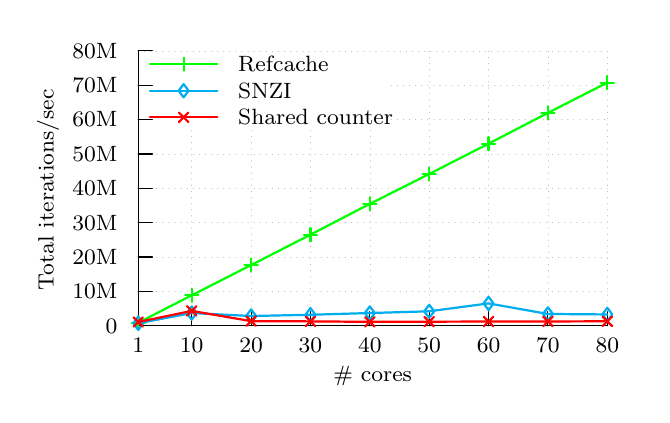
\begin{tikzpicture}[gnuplot]
%% generated with GNUPLOT 5.0p1 (Lua 5.3; terminal rev. 99, script rev. 100)
%% Tue  9 Feb 07:20:52 2016
\tikzset{every node/.append style={font={\fontsize{8.0pt}{9.6pt}\selectfont}}}
\path (0.000,0.000) rectangle (7.747,4.572);
\gpcolor{rgb color={0.753,0.753,0.753}}
\gpsetlinetype{gp lt axes}
\gpsetdashtype{gp dt axes}
\gpsetlinewidth{0.50}
\draw[gp path] (1.348,0.787)--(7.305,0.787);
\gpcolor{color=gp lt color border}
\gpsetlinetype{gp lt border}
\gpsetdashtype{gp dt solid}
\gpsetlinewidth{1.00}
\draw[gp path] (1.348,0.787)--(1.528,0.787);
\node[gp node right] at (1.201,0.787) {  0 };
\gpcolor{rgb color={0.753,0.753,0.753}}
\gpsetlinetype{gp lt axes}
\gpsetdashtype{gp dt axes}
\gpsetlinewidth{0.50}
\draw[gp path] (1.348,1.223)--(7.305,1.223);
\gpcolor{color=gp lt color border}
\gpsetlinetype{gp lt border}
\gpsetdashtype{gp dt solid}
\gpsetlinewidth{1.00}
\draw[gp path] (1.348,1.223)--(1.528,1.223);
\node[gp node right] at (1.201,1.223) {  10M};
\gpcolor{rgb color={0.753,0.753,0.753}}
\gpsetlinetype{gp lt axes}
\gpsetdashtype{gp dt axes}
\gpsetlinewidth{0.50}
\draw[gp path] (1.348,1.660)--(7.305,1.660);
\gpcolor{color=gp lt color border}
\gpsetlinetype{gp lt border}
\gpsetdashtype{gp dt solid}
\gpsetlinewidth{1.00}
\draw[gp path] (1.348,1.660)--(1.528,1.660);
\node[gp node right] at (1.201,1.660) {  20M};
\gpcolor{rgb color={0.753,0.753,0.753}}
\gpsetlinetype{gp lt axes}
\gpsetdashtype{gp dt axes}
\gpsetlinewidth{0.50}
\draw[gp path] (1.348,2.096)--(7.305,2.096);
\gpcolor{color=gp lt color border}
\gpsetlinetype{gp lt border}
\gpsetdashtype{gp dt solid}
\gpsetlinewidth{1.00}
\draw[gp path] (1.348,2.096)--(1.528,2.096);
\node[gp node right] at (1.201,2.096) {  30M};
\gpcolor{rgb color={0.753,0.753,0.753}}
\gpsetlinetype{gp lt axes}
\gpsetdashtype{gp dt axes}
\gpsetlinewidth{0.50}
\draw[gp path] (1.348,2.532)--(7.305,2.532);
\gpcolor{color=gp lt color border}
\gpsetlinetype{gp lt border}
\gpsetdashtype{gp dt solid}
\gpsetlinewidth{1.00}
\draw[gp path] (1.348,2.532)--(1.528,2.532);
\node[gp node right] at (1.201,2.532) {  40M};
\gpcolor{rgb color={0.753,0.753,0.753}}
\gpsetlinetype{gp lt axes}
\gpsetdashtype{gp dt axes}
\gpsetlinewidth{0.50}
\draw[gp path] (1.348,2.968)--(7.305,2.968);
\gpcolor{color=gp lt color border}
\gpsetlinetype{gp lt border}
\gpsetdashtype{gp dt solid}
\gpsetlinewidth{1.00}
\draw[gp path] (1.348,2.968)--(1.528,2.968);
\node[gp node right] at (1.201,2.968) {  50M};
\gpcolor{rgb color={0.753,0.753,0.753}}
\gpsetlinetype{gp lt axes}
\gpsetdashtype{gp dt axes}
\gpsetlinewidth{0.50}
\draw[gp path] (4.558,3.405)--(7.305,3.405);
\gpcolor{color=gp lt color border}
\gpsetlinetype{gp lt border}
\gpsetdashtype{gp dt solid}
\gpsetlinewidth{1.00}
\draw[gp path] (1.348,3.405)--(1.528,3.405);
\node[gp node right] at (1.201,3.405) {  60M};
\gpcolor{rgb color={0.753,0.753,0.753}}
\gpsetlinetype{gp lt axes}
\gpsetdashtype{gp dt axes}
\gpsetlinewidth{0.50}
\draw[gp path] (4.558,3.841)--(7.305,3.841);
\gpcolor{color=gp lt color border}
\gpsetlinetype{gp lt border}
\gpsetdashtype{gp dt solid}
\gpsetlinewidth{1.00}
\draw[gp path] (1.348,3.841)--(1.528,3.841);
\node[gp node right] at (1.201,3.841) {  70M};
\gpcolor{rgb color={0.753,0.753,0.753}}
\gpsetlinetype{gp lt axes}
\gpsetdashtype{gp dt axes}
\gpsetlinewidth{0.50}
\draw[gp path] (1.348,4.277)--(7.305,4.277);
\gpcolor{color=gp lt color border}
\gpsetlinetype{gp lt border}
\gpsetdashtype{gp dt solid}
\gpsetlinewidth{1.00}
\draw[gp path] (1.348,4.277)--(1.528,4.277);
\node[gp node right] at (1.201,4.277) {  80M};
\gpcolor{rgb color={0.753,0.753,0.753}}
\gpsetlinetype{gp lt axes}
\gpsetdashtype{gp dt axes}
\gpsetlinewidth{0.50}
\draw[gp path] (1.348,0.787)--(1.348,4.277);
\gpcolor{color=gp lt color border}
\gpsetlinetype{gp lt border}
\gpsetdashtype{gp dt solid}
\gpsetlinewidth{1.00}
\draw[gp path] (1.348,0.787)--(1.348,0.967);
\node[gp node center] at (1.348,0.541) {$1$};
\gpcolor{rgb color={0.753,0.753,0.753}}
\gpsetlinetype{gp lt axes}
\gpsetdashtype{gp dt axes}
\gpsetlinewidth{0.50}
\draw[gp path] (2.027,0.787)--(2.027,3.266);
\gpcolor{color=gp lt color border}
\gpsetlinetype{gp lt border}
\gpsetdashtype{gp dt solid}
\gpsetlinewidth{1.00}
\draw[gp path] (2.027,0.787)--(2.027,0.967);
\node[gp node center] at (2.027,0.541) {$10$};
\gpcolor{rgb color={0.753,0.753,0.753}}
\gpsetlinetype{gp lt axes}
\gpsetdashtype{gp dt axes}
\gpsetlinewidth{0.50}
\draw[gp path] (2.781,0.787)--(2.781,3.266);
\gpcolor{color=gp lt color border}
\gpsetlinetype{gp lt border}
\gpsetdashtype{gp dt solid}
\gpsetlinewidth{1.00}
\draw[gp path] (2.781,0.787)--(2.781,0.967);
\node[gp node center] at (2.781,0.541) {$20$};
\gpcolor{rgb color={0.753,0.753,0.753}}
\gpsetlinetype{gp lt axes}
\gpsetdashtype{gp dt axes}
\gpsetlinewidth{0.50}
\draw[gp path] (3.535,0.787)--(3.535,3.266);
\gpcolor{color=gp lt color border}
\gpsetlinetype{gp lt border}
\gpsetdashtype{gp dt solid}
\gpsetlinewidth{1.00}
\draw[gp path] (3.535,0.787)--(3.535,0.967);
\node[gp node center] at (3.535,0.541) {$30$};
\gpcolor{rgb color={0.753,0.753,0.753}}
\gpsetlinetype{gp lt axes}
\gpsetdashtype{gp dt axes}
\gpsetlinewidth{0.50}
\draw[gp path] (4.289,0.787)--(4.289,3.266);
\gpcolor{color=gp lt color border}
\gpsetlinetype{gp lt border}
\gpsetdashtype{gp dt solid}
\gpsetlinewidth{1.00}
\draw[gp path] (4.289,0.787)--(4.289,0.967);
\node[gp node center] at (4.289,0.541) {$40$};
\gpcolor{rgb color={0.753,0.753,0.753}}
\gpsetlinetype{gp lt axes}
\gpsetdashtype{gp dt axes}
\gpsetlinewidth{0.50}
\draw[gp path] (5.043,0.787)--(5.043,4.277);
\gpcolor{color=gp lt color border}
\gpsetlinetype{gp lt border}
\gpsetdashtype{gp dt solid}
\gpsetlinewidth{1.00}
\draw[gp path] (5.043,0.787)--(5.043,0.967);
\node[gp node center] at (5.043,0.541) {$50$};
\gpcolor{rgb color={0.753,0.753,0.753}}
\gpsetlinetype{gp lt axes}
\gpsetdashtype{gp dt axes}
\gpsetlinewidth{0.50}
\draw[gp path] (5.797,0.787)--(5.797,4.277);
\gpcolor{color=gp lt color border}
\gpsetlinetype{gp lt border}
\gpsetdashtype{gp dt solid}
\gpsetlinewidth{1.00}
\draw[gp path] (5.797,0.787)--(5.797,0.967);
\node[gp node center] at (5.797,0.541) {$60$};
\gpcolor{rgb color={0.753,0.753,0.753}}
\gpsetlinetype{gp lt axes}
\gpsetdashtype{gp dt axes}
\gpsetlinewidth{0.50}
\draw[gp path] (6.551,0.787)--(6.551,4.277);
\gpcolor{color=gp lt color border}
\gpsetlinetype{gp lt border}
\gpsetdashtype{gp dt solid}
\gpsetlinewidth{1.00}
\draw[gp path] (6.551,0.787)--(6.551,0.967);
\node[gp node center] at (6.551,0.541) {$70$};
\gpcolor{rgb color={0.753,0.753,0.753}}
\gpsetlinetype{gp lt axes}
\gpsetdashtype{gp dt axes}
\gpsetlinewidth{0.50}
\draw[gp path] (7.305,0.787)--(7.305,4.277);
\gpcolor{color=gp lt color border}
\gpsetlinetype{gp lt border}
\gpsetdashtype{gp dt solid}
\gpsetlinewidth{1.00}
\draw[gp path] (7.305,0.787)--(7.305,0.967);
\node[gp node center] at (7.305,0.541) {$80$};
\gpsetlinetype{gp lt axes}
\gpsetdashtype{gp dt axes}
\draw[gp path] (1.348,0.787)--(7.305,0.787);
\gpsetlinetype{gp lt border}
\gpsetdashtype{gp dt solid}
\draw[gp path] (1.348,4.277)--(1.348,0.787)--(7.305,0.787);
\node[gp node center,rotate=-270] at (0.196,2.532) {Total iterations/sec};
\node[gp node center] at (4.326,0.172) {\# cores};
\node[gp node left] at (2.500,4.108) {\refcache};
\gpcolor{color=gp lt color 1}
\gpsetlinewidth{2.00}
\draw[gp path] (1.495,4.108)--(2.353,4.108);
\draw[gp path] (1.348,0.825)--(2.027,1.173)--(2.781,1.557)--(3.535,1.943)--(4.289,2.334)%
  --(5.043,2.714)--(5.797,3.099)--(6.551,3.490)--(7.305,3.874);
\gpsetpointsize{6.00}
\gppoint{gp mark 1}{(1.348,0.825)}
\gppoint{gp mark 1}{(2.027,1.173)}
\gppoint{gp mark 1}{(2.781,1.557)}
\gppoint{gp mark 1}{(3.535,1.943)}
\gppoint{gp mark 1}{(4.289,2.334)}
\gppoint{gp mark 1}{(5.043,2.714)}
\gppoint{gp mark 1}{(5.797,3.099)}
\gppoint{gp mark 1}{(6.551,3.490)}
\gppoint{gp mark 1}{(7.305,3.874)}
\gppoint{gp mark 1}{(1.924,4.108)}
\gpcolor{color=gp lt color border}
\node[gp node left] at (2.500,3.771) {SNZI};
\gpcolor{color=gp lt color 4}
\draw[gp path] (1.495,3.771)--(2.353,3.771);
\draw[gp path] (1.348,0.818)--(2.027,0.948)--(2.781,0.910)--(3.535,0.926)--(4.289,0.948)%
  --(5.043,0.970)--(5.797,1.070)--(6.551,0.936)--(7.305,0.930);
\gppoint{gp mark 12}{(1.348,0.818)}
\gppoint{gp mark 12}{(2.027,0.948)}
\gppoint{gp mark 12}{(2.781,0.910)}
\gppoint{gp mark 12}{(3.535,0.926)}
\gppoint{gp mark 12}{(4.289,0.948)}
\gppoint{gp mark 12}{(5.043,0.970)}
\gppoint{gp mark 12}{(5.797,1.070)}
\gppoint{gp mark 12}{(6.551,0.936)}
\gppoint{gp mark 12}{(7.305,0.930)}
\gppoint{gp mark 12}{(1.924,3.771)}
\gpcolor{color=gp lt color border}
\node[gp node left] at (2.500,3.434) {Shared counter};
\gpcolor{color=gp lt color 0}
\draw[gp path] (1.495,3.434)--(2.353,3.434);
\draw[gp path] (1.348,0.834)--(2.027,0.975)--(2.781,0.845)--(3.535,0.842)--(4.289,0.836)%
  --(5.043,0.838)--(5.797,0.840)--(6.551,0.841)--(7.305,0.843);
\gppoint{gp mark 2}{(1.348,0.834)}
\gppoint{gp mark 2}{(2.027,0.975)}
\gppoint{gp mark 2}{(2.781,0.845)}
\gppoint{gp mark 2}{(3.535,0.842)}
\gppoint{gp mark 2}{(4.289,0.836)}
\gppoint{gp mark 2}{(5.043,0.838)}
\gppoint{gp mark 2}{(5.797,0.840)}
\gppoint{gp mark 2}{(6.551,0.841)}
\gppoint{gp mark 2}{(7.305,0.843)}
\gppoint{gp mark 2}{(1.924,3.434)}
%% coordinates of the plot area
\gpdefrectangularnode{gp plot 1}{\pgfpoint{1.348cm}{0.787cm}}{\pgfpoint{7.305cm}{4.277cm}}
\end{tikzpicture}
%% gnuplot variables
\\
        \vspace{1em}
        SNZI: Scalable Non-Zero Indicators
    \end{center}
    \end{column}
    \begin{column}{0.2\textwidth}
    \end{column}
  \end{columns}
\end{frame}

\begin{frame}{Question: Do we need targeted TLB shootdown?}
  \begin{center}
    Local microbenchmark, per-core versus shared\\
    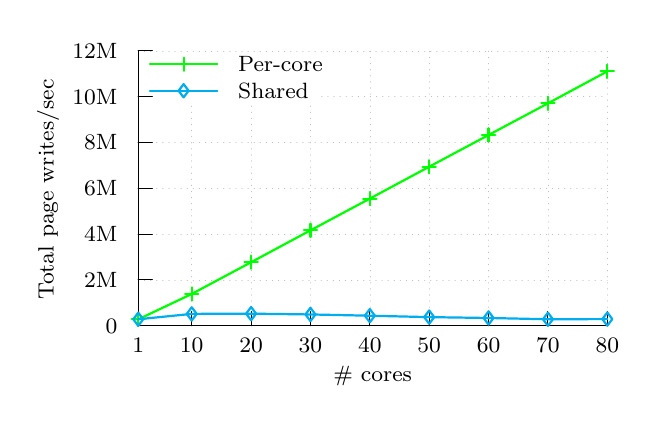
\begin{tikzpicture}[gnuplot]
%% generated with GNUPLOT 5.0p1 (Lua 5.3; terminal rev. 99, script rev. 100)
%% Tue  9 Feb 07:20:53 2016
\tikzset{every node/.append style={font={\fontsize{8.0pt}{9.6pt}\selectfont}}}
\path (0.000,0.000) rectangle (7.747,4.572);
\gpcolor{rgb color={0.753,0.753,0.753}}
\gpsetlinetype{gp lt axes}
\gpsetdashtype{gp dt axes}
\gpsetlinewidth{0.50}
\draw[gp path] (1.348,0.787)--(7.305,0.787);
\gpcolor{color=gp lt color border}
\gpsetlinetype{gp lt border}
\gpsetdashtype{gp dt solid}
\gpsetlinewidth{1.00}
\draw[gp path] (1.348,0.787)--(1.528,0.787);
\node[gp node right] at (1.201,0.787) {  0 };
\gpcolor{rgb color={0.753,0.753,0.753}}
\gpsetlinetype{gp lt axes}
\gpsetdashtype{gp dt axes}
\gpsetlinewidth{0.50}
\draw[gp path] (1.348,1.369)--(7.305,1.369);
\gpcolor{color=gp lt color border}
\gpsetlinetype{gp lt border}
\gpsetdashtype{gp dt solid}
\gpsetlinewidth{1.00}
\draw[gp path] (1.348,1.369)--(1.528,1.369);
\node[gp node right] at (1.201,1.369) {  2M};
\gpcolor{rgb color={0.753,0.753,0.753}}
\gpsetlinetype{gp lt axes}
\gpsetdashtype{gp dt axes}
\gpsetlinewidth{0.50}
\draw[gp path] (1.348,1.950)--(7.305,1.950);
\gpcolor{color=gp lt color border}
\gpsetlinetype{gp lt border}
\gpsetdashtype{gp dt solid}
\gpsetlinewidth{1.00}
\draw[gp path] (1.348,1.950)--(1.528,1.950);
\node[gp node right] at (1.201,1.950) {  4M};
\gpcolor{rgb color={0.753,0.753,0.753}}
\gpsetlinetype{gp lt axes}
\gpsetdashtype{gp dt axes}
\gpsetlinewidth{0.50}
\draw[gp path] (1.348,2.532)--(7.305,2.532);
\gpcolor{color=gp lt color border}
\gpsetlinetype{gp lt border}
\gpsetdashtype{gp dt solid}
\gpsetlinewidth{1.00}
\draw[gp path] (1.348,2.532)--(1.528,2.532);
\node[gp node right] at (1.201,2.532) {  6M};
\gpcolor{rgb color={0.753,0.753,0.753}}
\gpsetlinetype{gp lt axes}
\gpsetdashtype{gp dt axes}
\gpsetlinewidth{0.50}
\draw[gp path] (1.348,3.114)--(7.305,3.114);
\gpcolor{color=gp lt color border}
\gpsetlinetype{gp lt border}
\gpsetdashtype{gp dt solid}
\gpsetlinewidth{1.00}
\draw[gp path] (1.348,3.114)--(1.528,3.114);
\node[gp node right] at (1.201,3.114) {  8M};
\gpcolor{rgb color={0.753,0.753,0.753}}
\gpsetlinetype{gp lt axes}
\gpsetdashtype{gp dt axes}
\gpsetlinewidth{0.50}
\draw[gp path] (3.676,3.695)--(7.305,3.695);
\gpcolor{color=gp lt color border}
\gpsetlinetype{gp lt border}
\gpsetdashtype{gp dt solid}
\gpsetlinewidth{1.00}
\draw[gp path] (1.348,3.695)--(1.528,3.695);
\node[gp node right] at (1.201,3.695) {  10M};
\gpcolor{rgb color={0.753,0.753,0.753}}
\gpsetlinetype{gp lt axes}
\gpsetdashtype{gp dt axes}
\gpsetlinewidth{0.50}
\draw[gp path] (1.348,4.277)--(7.305,4.277);
\gpcolor{color=gp lt color border}
\gpsetlinetype{gp lt border}
\gpsetdashtype{gp dt solid}
\gpsetlinewidth{1.00}
\draw[gp path] (1.348,4.277)--(1.528,4.277);
\node[gp node right] at (1.201,4.277) {  12M};
\gpcolor{rgb color={0.753,0.753,0.753}}
\gpsetlinetype{gp lt axes}
\gpsetdashtype{gp dt axes}
\gpsetlinewidth{0.50}
\draw[gp path] (1.348,0.787)--(1.348,4.277);
\gpcolor{color=gp lt color border}
\gpsetlinetype{gp lt border}
\gpsetdashtype{gp dt solid}
\gpsetlinewidth{1.00}
\draw[gp path] (1.348,0.787)--(1.348,0.967);
\node[gp node center] at (1.348,0.541) {$1$};
\gpcolor{rgb color={0.753,0.753,0.753}}
\gpsetlinetype{gp lt axes}
\gpsetdashtype{gp dt axes}
\gpsetlinewidth{0.50}
\draw[gp path] (2.027,0.787)--(2.027,3.603);
\gpcolor{color=gp lt color border}
\gpsetlinetype{gp lt border}
\gpsetdashtype{gp dt solid}
\gpsetlinewidth{1.00}
\draw[gp path] (2.027,0.787)--(2.027,0.967);
\node[gp node center] at (2.027,0.541) {$10$};
\gpcolor{rgb color={0.753,0.753,0.753}}
\gpsetlinetype{gp lt axes}
\gpsetdashtype{gp dt axes}
\gpsetlinewidth{0.50}
\draw[gp path] (2.781,0.787)--(2.781,3.603);
\gpcolor{color=gp lt color border}
\gpsetlinetype{gp lt border}
\gpsetdashtype{gp dt solid}
\gpsetlinewidth{1.00}
\draw[gp path] (2.781,0.787)--(2.781,0.967);
\node[gp node center] at (2.781,0.541) {$20$};
\gpcolor{rgb color={0.753,0.753,0.753}}
\gpsetlinetype{gp lt axes}
\gpsetdashtype{gp dt axes}
\gpsetlinewidth{0.50}
\draw[gp path] (3.535,0.787)--(3.535,3.603);
\gpcolor{color=gp lt color border}
\gpsetlinetype{gp lt border}
\gpsetdashtype{gp dt solid}
\gpsetlinewidth{1.00}
\draw[gp path] (3.535,0.787)--(3.535,0.967);
\node[gp node center] at (3.535,0.541) {$30$};
\gpcolor{rgb color={0.753,0.753,0.753}}
\gpsetlinetype{gp lt axes}
\gpsetdashtype{gp dt axes}
\gpsetlinewidth{0.50}
\draw[gp path] (4.289,0.787)--(4.289,4.277);
\gpcolor{color=gp lt color border}
\gpsetlinetype{gp lt border}
\gpsetdashtype{gp dt solid}
\gpsetlinewidth{1.00}
\draw[gp path] (4.289,0.787)--(4.289,0.967);
\node[gp node center] at (4.289,0.541) {$40$};
\gpcolor{rgb color={0.753,0.753,0.753}}
\gpsetlinetype{gp lt axes}
\gpsetdashtype{gp dt axes}
\gpsetlinewidth{0.50}
\draw[gp path] (5.043,0.787)--(5.043,4.277);
\gpcolor{color=gp lt color border}
\gpsetlinetype{gp lt border}
\gpsetdashtype{gp dt solid}
\gpsetlinewidth{1.00}
\draw[gp path] (5.043,0.787)--(5.043,0.967);
\node[gp node center] at (5.043,0.541) {$50$};
\gpcolor{rgb color={0.753,0.753,0.753}}
\gpsetlinetype{gp lt axes}
\gpsetdashtype{gp dt axes}
\gpsetlinewidth{0.50}
\draw[gp path] (5.797,0.787)--(5.797,4.277);
\gpcolor{color=gp lt color border}
\gpsetlinetype{gp lt border}
\gpsetdashtype{gp dt solid}
\gpsetlinewidth{1.00}
\draw[gp path] (5.797,0.787)--(5.797,0.967);
\node[gp node center] at (5.797,0.541) {$60$};
\gpcolor{rgb color={0.753,0.753,0.753}}
\gpsetlinetype{gp lt axes}
\gpsetdashtype{gp dt axes}
\gpsetlinewidth{0.50}
\draw[gp path] (6.551,0.787)--(6.551,4.277);
\gpcolor{color=gp lt color border}
\gpsetlinetype{gp lt border}
\gpsetdashtype{gp dt solid}
\gpsetlinewidth{1.00}
\draw[gp path] (6.551,0.787)--(6.551,0.967);
\node[gp node center] at (6.551,0.541) {$70$};
\gpcolor{rgb color={0.753,0.753,0.753}}
\gpsetlinetype{gp lt axes}
\gpsetdashtype{gp dt axes}
\gpsetlinewidth{0.50}
\draw[gp path] (7.305,0.787)--(7.305,4.277);
\gpcolor{color=gp lt color border}
\gpsetlinetype{gp lt border}
\gpsetdashtype{gp dt solid}
\gpsetlinewidth{1.00}
\draw[gp path] (7.305,0.787)--(7.305,0.967);
\node[gp node center] at (7.305,0.541) {$80$};
\gpsetlinetype{gp lt axes}
\gpsetdashtype{gp dt axes}
\draw[gp path] (1.348,0.787)--(7.305,0.787);
\gpsetlinetype{gp lt border}
\gpsetdashtype{gp dt solid}
\draw[gp path] (1.348,4.277)--(1.348,0.787)--(7.305,0.787);
\node[gp node center,rotate=-270] at (0.196,2.532) {Total page writes/sec};
\node[gp node center] at (4.326,0.172) {\# cores};
\node[gp node left] at (2.500,4.108) {Per-core};
\gpcolor{color=gp lt color 1}
\gpsetlinewidth{2.00}
\draw[gp path] (1.495,4.108)--(2.353,4.108);
\draw[gp path] (1.348,0.868)--(2.027,1.190)--(2.781,1.593)--(3.535,1.998)--(4.289,2.401)%
  --(5.043,2.806)--(5.797,3.209)--(6.551,3.611)--(7.305,4.017);
\gpsetpointsize{6.00}
\gppoint{gp mark 1}{(1.348,0.868)}
\gppoint{gp mark 1}{(2.027,1.190)}
\gppoint{gp mark 1}{(2.781,1.593)}
\gppoint{gp mark 1}{(3.535,1.998)}
\gppoint{gp mark 1}{(4.289,2.401)}
\gppoint{gp mark 1}{(5.043,2.806)}
\gppoint{gp mark 1}{(5.797,3.209)}
\gppoint{gp mark 1}{(6.551,3.611)}
\gppoint{gp mark 1}{(7.305,4.017)}
\gppoint{gp mark 1}{(1.924,4.108)}
\gpcolor{color=gp lt color border}
\node[gp node left] at (2.500,3.771) {Shared};
\gpcolor{color=gp lt color 4}
\draw[gp path] (1.495,3.771)--(2.353,3.771);
\draw[gp path] (1.348,0.869)--(2.027,0.937)--(2.781,0.940)--(3.535,0.930)--(4.289,0.914)%
  --(5.043,0.896)--(5.797,0.885)--(6.551,0.869)--(7.305,0.871);
\gppoint{gp mark 12}{(1.348,0.869)}
\gppoint{gp mark 12}{(2.027,0.937)}
\gppoint{gp mark 12}{(2.781,0.940)}
\gppoint{gp mark 12}{(3.535,0.930)}
\gppoint{gp mark 12}{(4.289,0.914)}
\gppoint{gp mark 12}{(5.043,0.896)}
\gppoint{gp mark 12}{(5.797,0.885)}
\gppoint{gp mark 12}{(6.551,0.869)}
\gppoint{gp mark 12}{(7.305,0.871)}
\gppoint{gp mark 12}{(1.924,3.771)}
%% coordinates of the plot area
\gpdefrectangularnode{gp plot 1}{\pgfpoint{1.348cm}{0.787cm}}{\pgfpoint{7.305cm}{4.277cm}}
\end{tikzpicture}
%% gnuplot variables

  \end{center}
\end{frame}

\begin{frame}{Question: Do we need targeted TLB shootdown?}
  \begin{center}
    Pipeline microbenchmark, per-core versus shared\\
    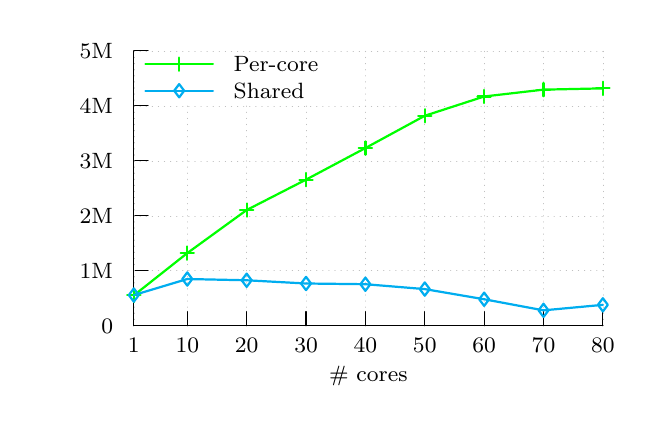
\begin{tikzpicture}[gnuplot]
%% generated with GNUPLOT 5.0p1 (Lua 5.3; terminal rev. 99, script rev. 100)
%% Tue  9 Feb 07:20:53 2016
\tikzset{every node/.append style={font={\fontsize{8.0pt}{9.6pt}\selectfont}}}
\path (0.000,0.000) rectangle (7.747,4.572);
\gpcolor{rgb color={0.753,0.753,0.753}}
\gpsetlinetype{gp lt axes}
\gpsetdashtype{gp dt axes}
\gpsetlinewidth{0.50}
\draw[gp path] (1.348,0.787)--(7.305,0.787);
\gpcolor{color=gp lt color border}
\gpsetlinetype{gp lt border}
\gpsetdashtype{gp dt solid}
\gpsetlinewidth{1.00}
\draw[gp path] (1.348,0.787)--(1.528,0.787);
\node[gp node right] at (1.201,0.787) {   0 };
\gpcolor{rgb color={0.753,0.753,0.753}}
\gpsetlinetype{gp lt axes}
\gpsetdashtype{gp dt axes}
\gpsetlinewidth{0.50}
\draw[gp path] (1.348,1.485)--(7.305,1.485);
\gpcolor{color=gp lt color border}
\gpsetlinetype{gp lt border}
\gpsetdashtype{gp dt solid}
\gpsetlinewidth{1.00}
\draw[gp path] (1.348,1.485)--(1.528,1.485);
\node[gp node right] at (1.201,1.485) {   1M};
\gpcolor{rgb color={0.753,0.753,0.753}}
\gpsetlinetype{gp lt axes}
\gpsetdashtype{gp dt axes}
\gpsetlinewidth{0.50}
\draw[gp path] (1.348,2.183)--(7.305,2.183);
\gpcolor{color=gp lt color border}
\gpsetlinetype{gp lt border}
\gpsetdashtype{gp dt solid}
\gpsetlinewidth{1.00}
\draw[gp path] (1.348,2.183)--(1.528,2.183);
\node[gp node right] at (1.201,2.183) {   2M};
\gpcolor{rgb color={0.753,0.753,0.753}}
\gpsetlinetype{gp lt axes}
\gpsetdashtype{gp dt axes}
\gpsetlinewidth{0.50}
\draw[gp path] (1.348,2.881)--(7.305,2.881);
\gpcolor{color=gp lt color border}
\gpsetlinetype{gp lt border}
\gpsetdashtype{gp dt solid}
\gpsetlinewidth{1.00}
\draw[gp path] (1.348,2.881)--(1.528,2.881);
\node[gp node right] at (1.201,2.881) {   3M};
\gpcolor{rgb color={0.753,0.753,0.753}}
\gpsetlinetype{gp lt axes}
\gpsetdashtype{gp dt axes}
\gpsetlinewidth{0.50}
\draw[gp path] (1.348,3.579)--(7.305,3.579);
\gpcolor{color=gp lt color border}
\gpsetlinetype{gp lt border}
\gpsetdashtype{gp dt solid}
\gpsetlinewidth{1.00}
\draw[gp path] (1.348,3.579)--(1.528,3.579);
\node[gp node right] at (1.201,3.579) {   4M};
\gpcolor{rgb color={0.753,0.753,0.753}}
\gpsetlinetype{gp lt axes}
\gpsetdashtype{gp dt axes}
\gpsetlinewidth{0.50}
\draw[gp path] (1.348,4.277)--(7.305,4.277);
\gpcolor{color=gp lt color border}
\gpsetlinetype{gp lt border}
\gpsetdashtype{gp dt solid}
\gpsetlinewidth{1.00}
\draw[gp path] (1.348,4.277)--(1.528,4.277);
\node[gp node right] at (1.201,4.277) {   5M};
\gpcolor{rgb color={0.753,0.753,0.753}}
\gpsetlinetype{gp lt axes}
\gpsetdashtype{gp dt axes}
\gpsetlinewidth{0.50}
\draw[gp path] (1.348,0.787)--(1.348,4.277);
\gpcolor{color=gp lt color border}
\gpsetlinetype{gp lt border}
\gpsetdashtype{gp dt solid}
\gpsetlinewidth{1.00}
\draw[gp path] (1.348,0.787)--(1.348,0.967);
\node[gp node center] at (1.348,0.541) {$1$};
\gpcolor{rgb color={0.753,0.753,0.753}}
\gpsetlinetype{gp lt axes}
\gpsetdashtype{gp dt axes}
\gpsetlinewidth{0.50}
\draw[gp path] (2.027,0.787)--(2.027,3.603);
\gpcolor{color=gp lt color border}
\gpsetlinetype{gp lt border}
\gpsetdashtype{gp dt solid}
\gpsetlinewidth{1.00}
\draw[gp path] (2.027,0.787)--(2.027,0.967);
\node[gp node center] at (2.027,0.541) {$10$};
\gpcolor{rgb color={0.753,0.753,0.753}}
\gpsetlinetype{gp lt axes}
\gpsetdashtype{gp dt axes}
\gpsetlinewidth{0.50}
\draw[gp path] (2.781,0.787)--(2.781,3.603);
\gpcolor{color=gp lt color border}
\gpsetlinetype{gp lt border}
\gpsetdashtype{gp dt solid}
\gpsetlinewidth{1.00}
\draw[gp path] (2.781,0.787)--(2.781,0.967);
\node[gp node center] at (2.781,0.541) {$20$};
\gpcolor{rgb color={0.753,0.753,0.753}}
\gpsetlinetype{gp lt axes}
\gpsetdashtype{gp dt axes}
\gpsetlinewidth{0.50}
\draw[gp path] (3.535,0.787)--(3.535,3.603);
\gpcolor{color=gp lt color border}
\gpsetlinetype{gp lt border}
\gpsetdashtype{gp dt solid}
\gpsetlinewidth{1.00}
\draw[gp path] (3.535,0.787)--(3.535,0.967);
\node[gp node center] at (3.535,0.541) {$30$};
\gpcolor{rgb color={0.753,0.753,0.753}}
\gpsetlinetype{gp lt axes}
\gpsetdashtype{gp dt axes}
\gpsetlinewidth{0.50}
\draw[gp path] (4.289,0.787)--(4.289,4.277);
\gpcolor{color=gp lt color border}
\gpsetlinetype{gp lt border}
\gpsetdashtype{gp dt solid}
\gpsetlinewidth{1.00}
\draw[gp path] (4.289,0.787)--(4.289,0.967);
\node[gp node center] at (4.289,0.541) {$40$};
\gpcolor{rgb color={0.753,0.753,0.753}}
\gpsetlinetype{gp lt axes}
\gpsetdashtype{gp dt axes}
\gpsetlinewidth{0.50}
\draw[gp path] (5.043,0.787)--(5.043,4.277);
\gpcolor{color=gp lt color border}
\gpsetlinetype{gp lt border}
\gpsetdashtype{gp dt solid}
\gpsetlinewidth{1.00}
\draw[gp path] (5.043,0.787)--(5.043,0.967);
\node[gp node center] at (5.043,0.541) {$50$};
\gpcolor{rgb color={0.753,0.753,0.753}}
\gpsetlinetype{gp lt axes}
\gpsetdashtype{gp dt axes}
\gpsetlinewidth{0.50}
\draw[gp path] (5.797,0.787)--(5.797,4.277);
\gpcolor{color=gp lt color border}
\gpsetlinetype{gp lt border}
\gpsetdashtype{gp dt solid}
\gpsetlinewidth{1.00}
\draw[gp path] (5.797,0.787)--(5.797,0.967);
\node[gp node center] at (5.797,0.541) {$60$};
\gpcolor{rgb color={0.753,0.753,0.753}}
\gpsetlinetype{gp lt axes}
\gpsetdashtype{gp dt axes}
\gpsetlinewidth{0.50}
\draw[gp path] (6.551,0.787)--(6.551,4.277);
\gpcolor{color=gp lt color border}
\gpsetlinetype{gp lt border}
\gpsetdashtype{gp dt solid}
\gpsetlinewidth{1.00}
\draw[gp path] (6.551,0.787)--(6.551,0.967);
\node[gp node center] at (6.551,0.541) {$70$};
\gpcolor{rgb color={0.753,0.753,0.753}}
\gpsetlinetype{gp lt axes}
\gpsetdashtype{gp dt axes}
\gpsetlinewidth{0.50}
\draw[gp path] (7.305,0.787)--(7.305,4.277);
\gpcolor{color=gp lt color border}
\gpsetlinetype{gp lt border}
\gpsetdashtype{gp dt solid}
\gpsetlinewidth{1.00}
\draw[gp path] (7.305,0.787)--(7.305,0.967);
\node[gp node center] at (7.305,0.541) {$80$};
\gpsetlinetype{gp lt axes}
\gpsetdashtype{gp dt axes}
\draw[gp path] (1.348,0.787)--(7.305,0.787);
\gpsetlinetype{gp lt border}
\gpsetdashtype{gp dt solid}
\draw[gp path] (1.348,4.277)--(1.348,0.787)--(7.305,0.787);
\node[gp node center,rotate=-270] at (0.196,2.532) {~};
\node[gp node center] at (4.326,0.172) {\# cores};
\node[gp node left] at (2.500,4.108) {Per-core};
\gpcolor{color=gp lt color 1}
\gpsetlinewidth{2.00}
\draw[gp path] (1.495,4.108)--(2.353,4.108);
\draw[gp path] (1.348,1.172)--(2.027,1.709)--(2.781,2.256)--(3.535,2.642)--(4.289,3.043)%
  --(5.043,3.453)--(5.797,3.698)--(6.551,3.785)--(7.305,3.801);
\gpsetpointsize{6.00}
\gppoint{gp mark 1}{(1.348,1.172)}
\gppoint{gp mark 1}{(2.027,1.709)}
\gppoint{gp mark 1}{(2.781,2.256)}
\gppoint{gp mark 1}{(3.535,2.642)}
\gppoint{gp mark 1}{(4.289,3.043)}
\gppoint{gp mark 1}{(5.043,3.453)}
\gppoint{gp mark 1}{(5.797,3.698)}
\gppoint{gp mark 1}{(6.551,3.785)}
\gppoint{gp mark 1}{(7.305,3.801)}
\gppoint{gp mark 1}{(1.924,4.108)}
\gpcolor{color=gp lt color border}
\node[gp node left] at (2.500,3.771) {Shared};
\gpcolor{color=gp lt color 4}
\draw[gp path] (1.495,3.771)--(2.353,3.771);
\draw[gp path] (1.348,1.176)--(2.027,1.380)--(2.781,1.364)--(3.535,1.323)--(4.289,1.314)%
  --(5.043,1.252)--(5.797,1.123)--(6.551,0.982)--(7.305,1.052);
\gppoint{gp mark 12}{(1.348,1.176)}
\gppoint{gp mark 12}{(2.027,1.380)}
\gppoint{gp mark 12}{(2.781,1.364)}
\gppoint{gp mark 12}{(3.535,1.323)}
\gppoint{gp mark 12}{(4.289,1.314)}
\gppoint{gp mark 12}{(5.043,1.252)}
\gppoint{gp mark 12}{(5.797,1.123)}
\gppoint{gp mark 12}{(6.551,0.982)}
\gppoint{gp mark 12}{(7.305,1.052)}
\gppoint{gp mark 12}{(1.924,3.771)}
%% coordinates of the plot area
\gpdefrectangularnode{gp plot 1}{\pgfpoint{1.348cm}{0.787cm}}{\pgfpoint{7.305cm}{4.277cm}}
\end{tikzpicture}
%% gnuplot variables

  \end{center}
\end{frame}

\begin{frame}{Question: Do we need targeted TLB shootdown?}
  \begin{center}
    Global microbenchmark, per-core versus shared\\
    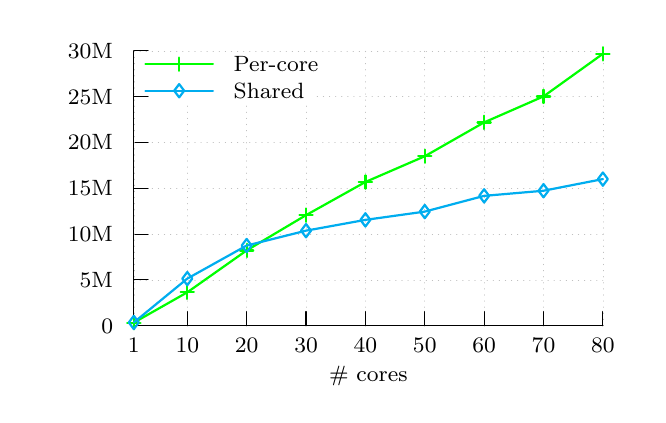
\begin{tikzpicture}[gnuplot]
%% generated with GNUPLOT 5.0p1 (Lua 5.3; terminal rev. 99, script rev. 100)
%% Tue  9 Feb 07:20:52 2016
\tikzset{every node/.append style={font={\fontsize{8.0pt}{9.6pt}\selectfont}}}
\path (0.000,0.000) rectangle (7.747,4.572);
\gpcolor{rgb color={0.753,0.753,0.753}}
\gpsetlinetype{gp lt axes}
\gpsetdashtype{gp dt axes}
\gpsetlinewidth{0.50}
\draw[gp path] (1.348,0.787)--(7.305,0.787);
\gpcolor{color=gp lt color border}
\gpsetlinetype{gp lt border}
\gpsetdashtype{gp dt solid}
\gpsetlinewidth{1.00}
\draw[gp path] (1.348,0.787)--(1.528,0.787);
\node[gp node right] at (1.201,0.787) {  0 };
\gpcolor{rgb color={0.753,0.753,0.753}}
\gpsetlinetype{gp lt axes}
\gpsetdashtype{gp dt axes}
\gpsetlinewidth{0.50}
\draw[gp path] (1.348,1.369)--(7.305,1.369);
\gpcolor{color=gp lt color border}
\gpsetlinetype{gp lt border}
\gpsetdashtype{gp dt solid}
\gpsetlinewidth{1.00}
\draw[gp path] (1.348,1.369)--(1.528,1.369);
\node[gp node right] at (1.201,1.369) {  5M};
\gpcolor{rgb color={0.753,0.753,0.753}}
\gpsetlinetype{gp lt axes}
\gpsetdashtype{gp dt axes}
\gpsetlinewidth{0.50}
\draw[gp path] (1.348,1.950)--(7.305,1.950);
\gpcolor{color=gp lt color border}
\gpsetlinetype{gp lt border}
\gpsetdashtype{gp dt solid}
\gpsetlinewidth{1.00}
\draw[gp path] (1.348,1.950)--(1.528,1.950);
\node[gp node right] at (1.201,1.950) {  10M};
\gpcolor{rgb color={0.753,0.753,0.753}}
\gpsetlinetype{gp lt axes}
\gpsetdashtype{gp dt axes}
\gpsetlinewidth{0.50}
\draw[gp path] (1.348,2.532)--(7.305,2.532);
\gpcolor{color=gp lt color border}
\gpsetlinetype{gp lt border}
\gpsetdashtype{gp dt solid}
\gpsetlinewidth{1.00}
\draw[gp path] (1.348,2.532)--(1.528,2.532);
\node[gp node right] at (1.201,2.532) {  15M};
\gpcolor{rgb color={0.753,0.753,0.753}}
\gpsetlinetype{gp lt axes}
\gpsetdashtype{gp dt axes}
\gpsetlinewidth{0.50}
\draw[gp path] (1.348,3.114)--(7.305,3.114);
\gpcolor{color=gp lt color border}
\gpsetlinetype{gp lt border}
\gpsetdashtype{gp dt solid}
\gpsetlinewidth{1.00}
\draw[gp path] (1.348,3.114)--(1.528,3.114);
\node[gp node right] at (1.201,3.114) {  20M};
\gpcolor{rgb color={0.753,0.753,0.753}}
\gpsetlinetype{gp lt axes}
\gpsetdashtype{gp dt axes}
\gpsetlinewidth{0.50}
\draw[gp path] (3.676,3.695)--(7.305,3.695);
\gpcolor{color=gp lt color border}
\gpsetlinetype{gp lt border}
\gpsetdashtype{gp dt solid}
\gpsetlinewidth{1.00}
\draw[gp path] (1.348,3.695)--(1.528,3.695);
\node[gp node right] at (1.201,3.695) {  25M};
\gpcolor{rgb color={0.753,0.753,0.753}}
\gpsetlinetype{gp lt axes}
\gpsetdashtype{gp dt axes}
\gpsetlinewidth{0.50}
\draw[gp path] (1.348,4.277)--(7.305,4.277);
\gpcolor{color=gp lt color border}
\gpsetlinetype{gp lt border}
\gpsetdashtype{gp dt solid}
\gpsetlinewidth{1.00}
\draw[gp path] (1.348,4.277)--(1.528,4.277);
\node[gp node right] at (1.201,4.277) {  30M};
\gpcolor{rgb color={0.753,0.753,0.753}}
\gpsetlinetype{gp lt axes}
\gpsetdashtype{gp dt axes}
\gpsetlinewidth{0.50}
\draw[gp path] (1.348,0.787)--(1.348,4.277);
\gpcolor{color=gp lt color border}
\gpsetlinetype{gp lt border}
\gpsetdashtype{gp dt solid}
\gpsetlinewidth{1.00}
\draw[gp path] (1.348,0.787)--(1.348,0.967);
\node[gp node center] at (1.348,0.541) {$1$};
\gpcolor{rgb color={0.753,0.753,0.753}}
\gpsetlinetype{gp lt axes}
\gpsetdashtype{gp dt axes}
\gpsetlinewidth{0.50}
\draw[gp path] (2.027,0.787)--(2.027,3.603);
\gpcolor{color=gp lt color border}
\gpsetlinetype{gp lt border}
\gpsetdashtype{gp dt solid}
\gpsetlinewidth{1.00}
\draw[gp path] (2.027,0.787)--(2.027,0.967);
\node[gp node center] at (2.027,0.541) {$10$};
\gpcolor{rgb color={0.753,0.753,0.753}}
\gpsetlinetype{gp lt axes}
\gpsetdashtype{gp dt axes}
\gpsetlinewidth{0.50}
\draw[gp path] (2.781,0.787)--(2.781,3.603);
\gpcolor{color=gp lt color border}
\gpsetlinetype{gp lt border}
\gpsetdashtype{gp dt solid}
\gpsetlinewidth{1.00}
\draw[gp path] (2.781,0.787)--(2.781,0.967);
\node[gp node center] at (2.781,0.541) {$20$};
\gpcolor{rgb color={0.753,0.753,0.753}}
\gpsetlinetype{gp lt axes}
\gpsetdashtype{gp dt axes}
\gpsetlinewidth{0.50}
\draw[gp path] (3.535,0.787)--(3.535,3.603);
\gpcolor{color=gp lt color border}
\gpsetlinetype{gp lt border}
\gpsetdashtype{gp dt solid}
\gpsetlinewidth{1.00}
\draw[gp path] (3.535,0.787)--(3.535,0.967);
\node[gp node center] at (3.535,0.541) {$30$};
\gpcolor{rgb color={0.753,0.753,0.753}}
\gpsetlinetype{gp lt axes}
\gpsetdashtype{gp dt axes}
\gpsetlinewidth{0.50}
\draw[gp path] (4.289,0.787)--(4.289,4.277);
\gpcolor{color=gp lt color border}
\gpsetlinetype{gp lt border}
\gpsetdashtype{gp dt solid}
\gpsetlinewidth{1.00}
\draw[gp path] (4.289,0.787)--(4.289,0.967);
\node[gp node center] at (4.289,0.541) {$40$};
\gpcolor{rgb color={0.753,0.753,0.753}}
\gpsetlinetype{gp lt axes}
\gpsetdashtype{gp dt axes}
\gpsetlinewidth{0.50}
\draw[gp path] (5.043,0.787)--(5.043,4.277);
\gpcolor{color=gp lt color border}
\gpsetlinetype{gp lt border}
\gpsetdashtype{gp dt solid}
\gpsetlinewidth{1.00}
\draw[gp path] (5.043,0.787)--(5.043,0.967);
\node[gp node center] at (5.043,0.541) {$50$};
\gpcolor{rgb color={0.753,0.753,0.753}}
\gpsetlinetype{gp lt axes}
\gpsetdashtype{gp dt axes}
\gpsetlinewidth{0.50}
\draw[gp path] (5.797,0.787)--(5.797,4.277);
\gpcolor{color=gp lt color border}
\gpsetlinetype{gp lt border}
\gpsetdashtype{gp dt solid}
\gpsetlinewidth{1.00}
\draw[gp path] (5.797,0.787)--(5.797,0.967);
\node[gp node center] at (5.797,0.541) {$60$};
\gpcolor{rgb color={0.753,0.753,0.753}}
\gpsetlinetype{gp lt axes}
\gpsetdashtype{gp dt axes}
\gpsetlinewidth{0.50}
\draw[gp path] (6.551,0.787)--(6.551,4.277);
\gpcolor{color=gp lt color border}
\gpsetlinetype{gp lt border}
\gpsetdashtype{gp dt solid}
\gpsetlinewidth{1.00}
\draw[gp path] (6.551,0.787)--(6.551,0.967);
\node[gp node center] at (6.551,0.541) {$70$};
\gpcolor{rgb color={0.753,0.753,0.753}}
\gpsetlinetype{gp lt axes}
\gpsetdashtype{gp dt axes}
\gpsetlinewidth{0.50}
\draw[gp path] (7.305,0.787)--(7.305,4.277);
\gpcolor{color=gp lt color border}
\gpsetlinetype{gp lt border}
\gpsetdashtype{gp dt solid}
\gpsetlinewidth{1.00}
\draw[gp path] (7.305,0.787)--(7.305,0.967);
\node[gp node center] at (7.305,0.541) {$80$};
\gpsetlinetype{gp lt axes}
\gpsetdashtype{gp dt axes}
\draw[gp path] (1.348,0.787)--(7.305,0.787);
\gpsetlinetype{gp lt border}
\gpsetdashtype{gp dt solid}
\draw[gp path] (1.348,4.277)--(1.348,0.787)--(7.305,0.787);
\node[gp node center,rotate=-270] at (0.196,2.532) {~};
\node[gp node center] at (4.326,0.172) {\# cores};
\node[gp node left] at (2.500,4.108) {Per-core};
\gpcolor{color=gp lt color 1}
\gpsetlinewidth{2.00}
\draw[gp path] (1.495,4.108)--(2.353,4.108);
\draw[gp path] (1.348,0.826)--(2.027,1.211)--(2.781,1.743)--(3.535,2.191)--(4.289,2.612)%
  --(5.043,2.939)--(5.797,3.369)--(6.551,3.699)--(7.305,4.240);
\gpsetpointsize{6.00}
\gppoint{gp mark 1}{(1.348,0.826)}
\gppoint{gp mark 1}{(2.027,1.211)}
\gppoint{gp mark 1}{(2.781,1.743)}
\gppoint{gp mark 1}{(3.535,2.191)}
\gppoint{gp mark 1}{(4.289,2.612)}
\gppoint{gp mark 1}{(5.043,2.939)}
\gppoint{gp mark 1}{(5.797,3.369)}
\gppoint{gp mark 1}{(6.551,3.699)}
\gppoint{gp mark 1}{(7.305,4.240)}
\gppoint{gp mark 1}{(1.924,4.108)}
\gpcolor{color=gp lt color border}
\node[gp node left] at (2.500,3.771) {Shared};
\gpcolor{color=gp lt color 4}
\draw[gp path] (1.495,3.771)--(2.353,3.771);
\draw[gp path] (1.348,0.828)--(2.027,1.385)--(2.781,1.805)--(3.535,1.994)--(4.289,2.131)%
  --(5.043,2.236)--(5.797,2.436)--(6.551,2.501)--(7.305,2.649);
\gppoint{gp mark 12}{(1.348,0.828)}
\gppoint{gp mark 12}{(2.027,1.385)}
\gppoint{gp mark 12}{(2.781,1.805)}
\gppoint{gp mark 12}{(3.535,1.994)}
\gppoint{gp mark 12}{(4.289,2.131)}
\gppoint{gp mark 12}{(5.043,2.236)}
\gppoint{gp mark 12}{(5.797,2.436)}
\gppoint{gp mark 12}{(6.551,2.501)}
\gppoint{gp mark 12}{(7.305,2.649)}
\gppoint{gp mark 12}{(1.924,3.771)}
%% coordinates of the plot area
\gpdefrectangularnode{gp plot 1}{\pgfpoint{1.348cm}{0.787cm}}{\pgfpoint{7.305cm}{4.277cm}}
\end{tikzpicture}
%% gnuplot variables

  \end{center}
\end{frame}

\begin{frame}{Issue: Memory Overhead}
  \begin{center}
    \begin{tabular}{ l | c | c c | c }
              &        & \multicolumn{2}{c|}{Linux} & Radix tree \\
              & RSS    & VMA tree & Page table      & (rel. to Linux) \\
      \hline
      Firefox & 352 MB & 117 KB   & 1.5 MB          & 3.9 MB (2.4$\times$) \\
      Chrome  & 152 MB & 124 KB   & 1.1 MB          & 2.4 MB (2.0$\times$) \\
      Apache  & 16 MB  & 44 KB    & 368 KB          & 616 KB (1.5$\times$) \\
      MySQL   & 84 MB  & 18 KB    & 348 KB          & 980 KB (2.7$\times$) \\
    \end{tabular}
    \vspace{1em}
    \bi
  \item RSS
    \bi
  \item Resident Set Size
  \item physical memory used by a process
    \ei
  \item VMA
    \bi
  \item Virtual Memory Areas
  \item stored in a red-black tree in Linux
    \ei
    \ei
  \end{center}
\end{frame}

\begin{frame}{Summary}
  \begin{columns}[T]
    \begin{column}{0.5\textwidth}
      \begin{center}
        Metis performance\\
        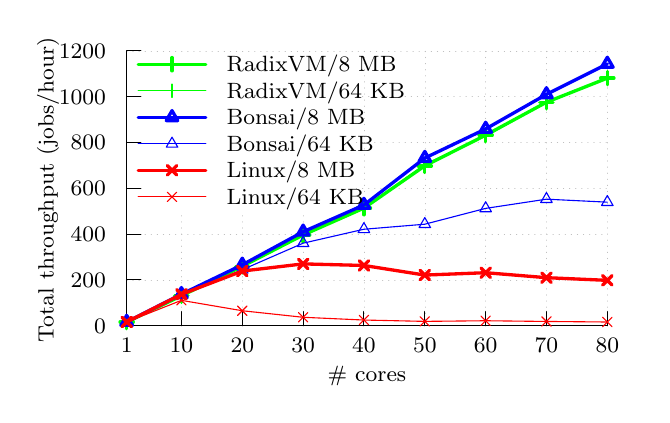
\begin{tikzpicture}[gnuplot]
%% generated with GNUPLOT 5.0p1 (Lua 5.3; terminal rev. 99, script rev. 100)
%% Tue  9 Feb 07:19:36 2016
\tikzset{every node/.append style={font={\fontsize{8.0pt}{9.6pt}\selectfont}}}
\path (0.000,0.000) rectangle (7.747,4.572);
\gpcolor{rgb color={0.753,0.753,0.753}}
\gpsetlinetype{gp lt axes}
\gpsetdashtype{gp dt axes}
\gpsetlinewidth{0.50}
\draw[gp path] (1.201,0.787)--(7.305,0.787);
\gpcolor{color=gp lt color border}
\gpsetlinetype{gp lt border}
\gpsetdashtype{gp dt solid}
\gpsetlinewidth{1.00}
\draw[gp path] (1.201,0.787)--(1.381,0.787);
\node[gp node right] at (1.054,0.787) {$0$};
\gpcolor{rgb color={0.753,0.753,0.753}}
\gpsetlinetype{gp lt axes}
\gpsetdashtype{gp dt axes}
\gpsetlinewidth{0.50}
\draw[gp path] (1.201,1.369)--(7.305,1.369);
\gpcolor{color=gp lt color border}
\gpsetlinetype{gp lt border}
\gpsetdashtype{gp dt solid}
\gpsetlinewidth{1.00}
\draw[gp path] (1.201,1.369)--(1.381,1.369);
\node[gp node right] at (1.054,1.369) {$200$};
\gpcolor{rgb color={0.753,0.753,0.753}}
\gpsetlinetype{gp lt axes}
\gpsetdashtype{gp dt axes}
\gpsetlinewidth{0.50}
\draw[gp path] (1.201,1.950)--(7.305,1.950);
\gpcolor{color=gp lt color border}
\gpsetlinetype{gp lt border}
\gpsetdashtype{gp dt solid}
\gpsetlinewidth{1.00}
\draw[gp path] (1.201,1.950)--(1.381,1.950);
\node[gp node right] at (1.054,1.950) {$400$};
\gpcolor{rgb color={0.753,0.753,0.753}}
\gpsetlinetype{gp lt axes}
\gpsetdashtype{gp dt axes}
\gpsetlinewidth{0.50}
\draw[gp path] (4.117,2.532)--(7.305,2.532);
\gpcolor{color=gp lt color border}
\gpsetlinetype{gp lt border}
\gpsetdashtype{gp dt solid}
\gpsetlinewidth{1.00}
\draw[gp path] (1.201,2.532)--(1.381,2.532);
\node[gp node right] at (1.054,2.532) {$600$};
\gpcolor{rgb color={0.753,0.753,0.753}}
\gpsetlinetype{gp lt axes}
\gpsetdashtype{gp dt axes}
\gpsetlinewidth{0.50}
\draw[gp path] (4.117,3.114)--(7.305,3.114);
\gpcolor{color=gp lt color border}
\gpsetlinetype{gp lt border}
\gpsetdashtype{gp dt solid}
\gpsetlinewidth{1.00}
\draw[gp path] (1.201,3.114)--(1.381,3.114);
\node[gp node right] at (1.054,3.114) {$800$};
\gpcolor{rgb color={0.753,0.753,0.753}}
\gpsetlinetype{gp lt axes}
\gpsetdashtype{gp dt axes}
\gpsetlinewidth{0.50}
\draw[gp path] (4.117,3.695)--(7.305,3.695);
\gpcolor{color=gp lt color border}
\gpsetlinetype{gp lt border}
\gpsetdashtype{gp dt solid}
\gpsetlinewidth{1.00}
\draw[gp path] (1.201,3.695)--(1.381,3.695);
\node[gp node right] at (1.054,3.695) {$1000$};
\gpcolor{rgb color={0.753,0.753,0.753}}
\gpsetlinetype{gp lt axes}
\gpsetdashtype{gp dt axes}
\gpsetlinewidth{0.50}
\draw[gp path] (1.201,4.277)--(7.305,4.277);
\gpcolor{color=gp lt color border}
\gpsetlinetype{gp lt border}
\gpsetdashtype{gp dt solid}
\gpsetlinewidth{1.00}
\draw[gp path] (1.201,4.277)--(1.381,4.277);
\node[gp node right] at (1.054,4.277) {$1200$};
\gpcolor{rgb color={0.753,0.753,0.753}}
\gpsetlinetype{gp lt axes}
\gpsetdashtype{gp dt axes}
\gpsetlinewidth{0.50}
\draw[gp path] (1.201,0.787)--(1.201,4.277);
\gpcolor{color=gp lt color border}
\gpsetlinetype{gp lt border}
\gpsetdashtype{gp dt solid}
\gpsetlinewidth{1.00}
\draw[gp path] (1.201,0.787)--(1.201,0.967);
\node[gp node center] at (1.201,0.541) {$1$};
\gpcolor{rgb color={0.753,0.753,0.753}}
\gpsetlinetype{gp lt axes}
\gpsetdashtype{gp dt axes}
\gpsetlinewidth{0.50}
\draw[gp path] (1.896,0.787)--(1.896,2.255);
\gpcolor{color=gp lt color border}
\gpsetlinetype{gp lt border}
\gpsetdashtype{gp dt solid}
\gpsetlinewidth{1.00}
\draw[gp path] (1.896,0.787)--(1.896,0.967);
\node[gp node center] at (1.896,0.541) {$10$};
\gpcolor{rgb color={0.753,0.753,0.753}}
\gpsetlinetype{gp lt axes}
\gpsetdashtype{gp dt axes}
\gpsetlinewidth{0.50}
\draw[gp path] (2.669,0.787)--(2.669,2.255);
\gpcolor{color=gp lt color border}
\gpsetlinetype{gp lt border}
\gpsetdashtype{gp dt solid}
\gpsetlinewidth{1.00}
\draw[gp path] (2.669,0.787)--(2.669,0.967);
\node[gp node center] at (2.669,0.541) {$20$};
\gpcolor{rgb color={0.753,0.753,0.753}}
\gpsetlinetype{gp lt axes}
\gpsetdashtype{gp dt axes}
\gpsetlinewidth{0.50}
\draw[gp path] (3.442,0.787)--(3.442,2.255);
\gpcolor{color=gp lt color border}
\gpsetlinetype{gp lt border}
\gpsetdashtype{gp dt solid}
\gpsetlinewidth{1.00}
\draw[gp path] (3.442,0.787)--(3.442,0.967);
\node[gp node center] at (3.442,0.541) {$30$};
\gpcolor{rgb color={0.753,0.753,0.753}}
\gpsetlinetype{gp lt axes}
\gpsetdashtype{gp dt axes}
\gpsetlinewidth{0.50}
\draw[gp path] (4.214,0.787)--(4.214,4.277);
\gpcolor{color=gp lt color border}
\gpsetlinetype{gp lt border}
\gpsetdashtype{gp dt solid}
\gpsetlinewidth{1.00}
\draw[gp path] (4.214,0.787)--(4.214,0.967);
\node[gp node center] at (4.214,0.541) {$40$};
\gpcolor{rgb color={0.753,0.753,0.753}}
\gpsetlinetype{gp lt axes}
\gpsetdashtype{gp dt axes}
\gpsetlinewidth{0.50}
\draw[gp path] (4.987,0.787)--(4.987,4.277);
\gpcolor{color=gp lt color border}
\gpsetlinetype{gp lt border}
\gpsetdashtype{gp dt solid}
\gpsetlinewidth{1.00}
\draw[gp path] (4.987,0.787)--(4.987,0.967);
\node[gp node center] at (4.987,0.541) {$50$};
\gpcolor{rgb color={0.753,0.753,0.753}}
\gpsetlinetype{gp lt axes}
\gpsetdashtype{gp dt axes}
\gpsetlinewidth{0.50}
\draw[gp path] (5.760,0.787)--(5.760,4.277);
\gpcolor{color=gp lt color border}
\gpsetlinetype{gp lt border}
\gpsetdashtype{gp dt solid}
\gpsetlinewidth{1.00}
\draw[gp path] (5.760,0.787)--(5.760,0.967);
\node[gp node center] at (5.760,0.541) {$60$};
\gpcolor{rgb color={0.753,0.753,0.753}}
\gpsetlinetype{gp lt axes}
\gpsetdashtype{gp dt axes}
\gpsetlinewidth{0.50}
\draw[gp path] (6.532,0.787)--(6.532,4.277);
\gpcolor{color=gp lt color border}
\gpsetlinetype{gp lt border}
\gpsetdashtype{gp dt solid}
\gpsetlinewidth{1.00}
\draw[gp path] (6.532,0.787)--(6.532,0.967);
\node[gp node center] at (6.532,0.541) {$70$};
\gpcolor{rgb color={0.753,0.753,0.753}}
\gpsetlinetype{gp lt axes}
\gpsetdashtype{gp dt axes}
\gpsetlinewidth{0.50}
\draw[gp path] (7.305,0.787)--(7.305,4.277);
\gpcolor{color=gp lt color border}
\gpsetlinetype{gp lt border}
\gpsetdashtype{gp dt solid}
\gpsetlinewidth{1.00}
\draw[gp path] (7.305,0.787)--(7.305,0.967);
\node[gp node center] at (7.305,0.541) {$80$};
\gpsetlinetype{gp lt axes}
\gpsetdashtype{gp dt axes}
\draw[gp path] (1.201,0.787)--(7.305,0.787);
\gpsetlinetype{gp lt border}
\gpsetdashtype{gp dt solid}
\draw[gp path] (1.201,4.277)--(1.201,0.787)--(7.305,0.787);
\node[gp node center,rotate=-270] at (0.196,2.532) {Total throughput (jobs/hour)};
\node[gp node center] at (4.253,0.172) {\# cores};
\node[gp node left] at (2.353,4.108) {\vm/8~MB};
\gpcolor{color=gp lt color 1}
\gpsetlinewidth{3.00}
\draw[gp path] (1.348,4.108)--(2.206,4.108);
\draw[gp path] (1.201,0.833)--(1.896,1.167)--(2.669,1.541)--(3.442,1.939)--(4.214,2.280)%
  --(4.987,2.817)--(5.760,3.207)--(6.532,3.625)--(7.305,3.931);
\gpsetpointsize{6.00}
\gppoint{gp mark 1}{(1.201,0.833)}
\gppoint{gp mark 1}{(1.896,1.167)}
\gppoint{gp mark 1}{(2.669,1.541)}
\gppoint{gp mark 1}{(3.442,1.939)}
\gppoint{gp mark 1}{(4.214,2.280)}
\gppoint{gp mark 1}{(4.987,2.817)}
\gppoint{gp mark 1}{(5.760,3.207)}
\gppoint{gp mark 1}{(6.532,3.625)}
\gppoint{gp mark 1}{(7.305,3.931)}
\gppoint{gp mark 1}{(1.777,4.108)}
\gpcolor{color=gp lt color border}
\node[gp node left] at (2.353,3.771) {\vm/64~KB};
\gpcolor{color=gp lt color 1}
\gpsetlinewidth{1.00}
\draw[gp path] (1.348,3.771)--(2.206,3.771);
\draw[gp path] (1.201,0.833)--(1.896,1.169)--(2.669,1.541)--(3.442,1.937)--(4.214,2.279)%
  --(4.987,2.836)--(5.760,3.193)--(6.532,3.618)--(7.305,3.926);
\gppoint{gp mark 1}{(1.201,0.833)}
\gppoint{gp mark 1}{(1.896,1.169)}
\gppoint{gp mark 1}{(2.669,1.541)}
\gppoint{gp mark 1}{(3.442,1.937)}
\gppoint{gp mark 1}{(4.214,2.279)}
\gppoint{gp mark 1}{(4.987,2.836)}
\gppoint{gp mark 1}{(5.760,3.193)}
\gppoint{gp mark 1}{(6.532,3.618)}
\gppoint{gp mark 1}{(7.305,3.926)}
\gppoint{gp mark 1}{(1.777,3.771)}
\gpcolor{color=gp lt color border}
\node[gp node left] at (2.353,3.434) {Bonsai/8~MB};
\gpcolor{color=gp lt color 2}
\gpsetlinewidth{3.00}
\draw[gp path] (1.348,3.434)--(2.206,3.434);
\draw[gp path] (1.201,0.834)--(1.896,1.187)--(2.669,1.560)--(3.442,1.980)--(4.214,2.320)%
  --(4.987,2.916)--(5.760,3.286)--(6.532,3.725)--(7.305,4.112);
\gppoint{gp mark 8}{(1.201,0.834)}
\gppoint{gp mark 8}{(1.896,1.187)}
\gppoint{gp mark 8}{(2.669,1.560)}
\gppoint{gp mark 8}{(3.442,1.980)}
\gppoint{gp mark 8}{(4.214,2.320)}
\gppoint{gp mark 8}{(4.987,2.916)}
\gppoint{gp mark 8}{(5.760,3.286)}
\gppoint{gp mark 8}{(6.532,3.725)}
\gppoint{gp mark 8}{(7.305,4.112)}
\gppoint{gp mark 8}{(1.777,3.434)}
\gpcolor{color=gp lt color border}
\node[gp node left] at (2.353,3.097) {Bonsai/64~KB};
\gpcolor{color=gp lt color 2}
\gpsetlinewidth{1.00}
\draw[gp path] (1.348,3.097)--(2.206,3.097);
\draw[gp path] (1.201,0.834)--(1.896,1.174)--(2.669,1.498)--(3.442,1.835)--(4.214,2.012)%
  --(4.987,2.076)--(5.760,2.277)--(6.532,2.394)--(7.305,2.356);
\gppoint{gp mark 8}{(1.201,0.834)}
\gppoint{gp mark 8}{(1.896,1.174)}
\gppoint{gp mark 8}{(2.669,1.498)}
\gppoint{gp mark 8}{(3.442,1.835)}
\gppoint{gp mark 8}{(4.214,2.012)}
\gppoint{gp mark 8}{(4.987,2.076)}
\gppoint{gp mark 8}{(5.760,2.277)}
\gppoint{gp mark 8}{(6.532,2.394)}
\gppoint{gp mark 8}{(7.305,2.356)}
\gppoint{gp mark 8}{(1.777,3.097)}
\gpcolor{color=gp lt color border}
\node[gp node left] at (2.353,2.760) {Linux/8~MB};
\gpcolor{color=gp lt color 0}
\gpsetlinewidth{3.00}
\draw[gp path] (1.348,2.760)--(2.206,2.760);
\draw[gp path] (1.201,0.834)--(1.896,1.185)--(2.669,1.481)--(3.442,1.572)--(4.214,1.552)%
  --(4.987,1.430)--(5.760,1.460)--(6.532,1.397)--(7.305,1.363);
\gppoint{gp mark 2}{(1.201,0.834)}
\gppoint{gp mark 2}{(1.896,1.185)}
\gppoint{gp mark 2}{(2.669,1.481)}
\gppoint{gp mark 2}{(3.442,1.572)}
\gppoint{gp mark 2}{(4.214,1.552)}
\gppoint{gp mark 2}{(4.987,1.430)}
\gppoint{gp mark 2}{(5.760,1.460)}
\gppoint{gp mark 2}{(6.532,1.397)}
\gppoint{gp mark 2}{(7.305,1.363)}
\gppoint{gp mark 2}{(1.777,2.760)}
\gpcolor{color=gp lt color border}
\node[gp node left] at (2.353,2.423) {Linux/64~KB};
\gpcolor{color=gp lt color 0}
\gpsetlinewidth{1.00}
\draw[gp path] (1.348,2.423)--(2.206,2.423);
\draw[gp path] (1.201,0.834)--(1.896,1.109)--(2.669,0.977)--(3.442,0.894)--(4.214,0.859)%
  --(4.987,0.842)--(5.760,0.850)--(6.532,0.841)--(7.305,0.834);
\gppoint{gp mark 2}{(1.201,0.834)}
\gppoint{gp mark 2}{(1.896,1.109)}
\gppoint{gp mark 2}{(2.669,0.977)}
\gppoint{gp mark 2}{(3.442,0.894)}
\gppoint{gp mark 2}{(4.214,0.859)}
\gppoint{gp mark 2}{(4.987,0.842)}
\gppoint{gp mark 2}{(5.760,0.850)}
\gppoint{gp mark 2}{(6.532,0.841)}
\gppoint{gp mark 2}{(7.305,0.834)}
\gppoint{gp mark 2}{(1.777,2.423)}
%% coordinates of the plot area
\gpdefrectangularnode{gp plot 1}{\pgfpoint{1.201cm}{0.787cm}}{\pgfpoint{7.305cm}{4.277cm}}
\end{tikzpicture}
%% gnuplot variables

      \end{center}
    \end{column}
    \begin{column}{0.5\textwidth}
      \bi
    \item {\color{green}Good}: Scales well on
      \bi
    \item Metis, real-world application
    \item Microbenchmarks
      \ei
    \item {\color{red}Bad}: Increased memory overhead
      \ei
    \begin{tabular}{ l | c | c | c }
              &        &         & Radix tree \\
              & RSS    & Linux   & (rel. to Linux) \\
      \hline
      Firefox & 352 MB & 1.5 MB  & 3.9 MB (2.4$\times$) \\
      Chrome  & 152 MB & 1.1 MB  & 2.4 MB (2.0$\times$) \\
      Apache  & 16 MB  & 368 KB  & 616 KB (1.5$\times$) \\
      MySQL   & 84 MB  & 348 KB  & 980 KB (2.7$\times$) \\
    \end{tabular}
    \end{column}
  \end{columns}
\end{frame}

\begin{frame}[noframenumbering]{References}
  \bi
\item Clements, Austin T., M. Frans Kaashoek, and Nickolai Zeldovich. "RadixVM: Scalable address spaces for multithreaded applications." In \emph{Proceedings of the 8th ACM European Conference on Computer Systems}, pp. 211-224. ACM, 2013.
  \bi
\item Revised version: \url{https://pdos.csail.mit.edu/papers/radixvm:eurosys13-2014-08-05.pdf}
  \ei
\item 6.828 Lecture on RadixVM:\\
  \url{https://www.youtube.com/watch?v=qlg7jqBtR4c}
\item Clements, Austin T., M. Frans Kaashoek, and Nickolai Zeldovich. "Scalable address spaces using RCU balanced trees." \emph{ACM SIGPLAN Notices} 47, no. 4 (2012): 199-210.
  \bi
\item Available online: \url{https://pdos.csail.mit.edu/papers/rcuvm:asplos12.pdf}
  \ei
\item Linux VM info from:\\ \url{http://duartes.org/gustavo/blog/post/how-the-kernel-manages-your-memory/}
  \ei
\end{frame}

\begin{frame}[noframenumbering]{Attribution}
  \bi
  {\small
\item Refcache diagram, radix data structure diagram, and RadixVM charts used with permission by Austin Clements
\item Virtual memory diagram by Ehamberg (Own work) [CC BY-SA 3.0 (\url{http://creativecommons.org/licenses/by-sa/3.0})], via Wikimedia Commons
  \item MMU diagram by Mdjango, Andrew S. Tanenbaum (Own work) [CC BY-SA 3.0 (\url{http://creativecommons.org/licenses/by-sa/3.0})], via Wikimedia Commons
\item Address space diagram by Majenko (Own work) [CC BY-SA 4.0 (\url{http://creativecommons.org/licenses/by-sa/4.0})], via Wikimedia Commons
\item Patricia trie diagram by Saffles (Microsoft Visio) [CC BY-SA 3.0 (\url{http://creativecommons.org/licenses/by-sa/3.0})], via Wikimedia Commons
  \item Binary tree rotation diagram by Josell7 (Own work) [CC BY-SA 3.0 (\url{http://creativecommons.org/licenses/by-sa/3.0})], via Wikimedia Commons}
  \ei
\end{frame}

\begin{frame}[noframenumbering]{License}
  \bi
\item These slides are distributed under the creative commons
  Attribution-ShareAlike 4.0 International (CC BY-SA 4.0).
\item See http://creativecommons.org/licenses/by-sa/4.0/ for details.
  \ei
\end{frame}

\end{document}
